\section{Introduction}

The ERGM results presented in Chapter \ref{chp:ergm_result} address the empirical domain in our critical realist framework, namely the observed or measured network effects. We now need to account for unobserved or actual reality, specifically the hidden mechanisms and structures that drive or influence social interaction in our three open innovation partnerships \citep{welch2011theorising, mcavoy2018critical, haigh2019developing}. This chapter reports on the qualitative analysis of semi-structured interview transcripts. Unlike the ERGM analysis, which employs deductive logic to test propositions about social interactions, the qualitative analysis uses first- and second-cycle coding to unpack the interacting causal mechanisms that shape tacit knowledge sharing relations in our three open innovation partnerships. First-cycle coding employs inductive logic to expand a set of provisional codes derived from the propositions into sub-codes that unpack how different social mechanisms operate in practice (Table \ref{tab:provcode3}). Second-cycle coding uses the logic of retroduction to group the sub-codes into categorical codes. In this study, the categorical codes align with the main components of \citeauthor{loyal2001agency}'s \citeyearpar{loyal2001agency} agency model (Figure \ref{fig:agency_structure3}). \medskip

\begin{figure}[hbt!]
    \centering
    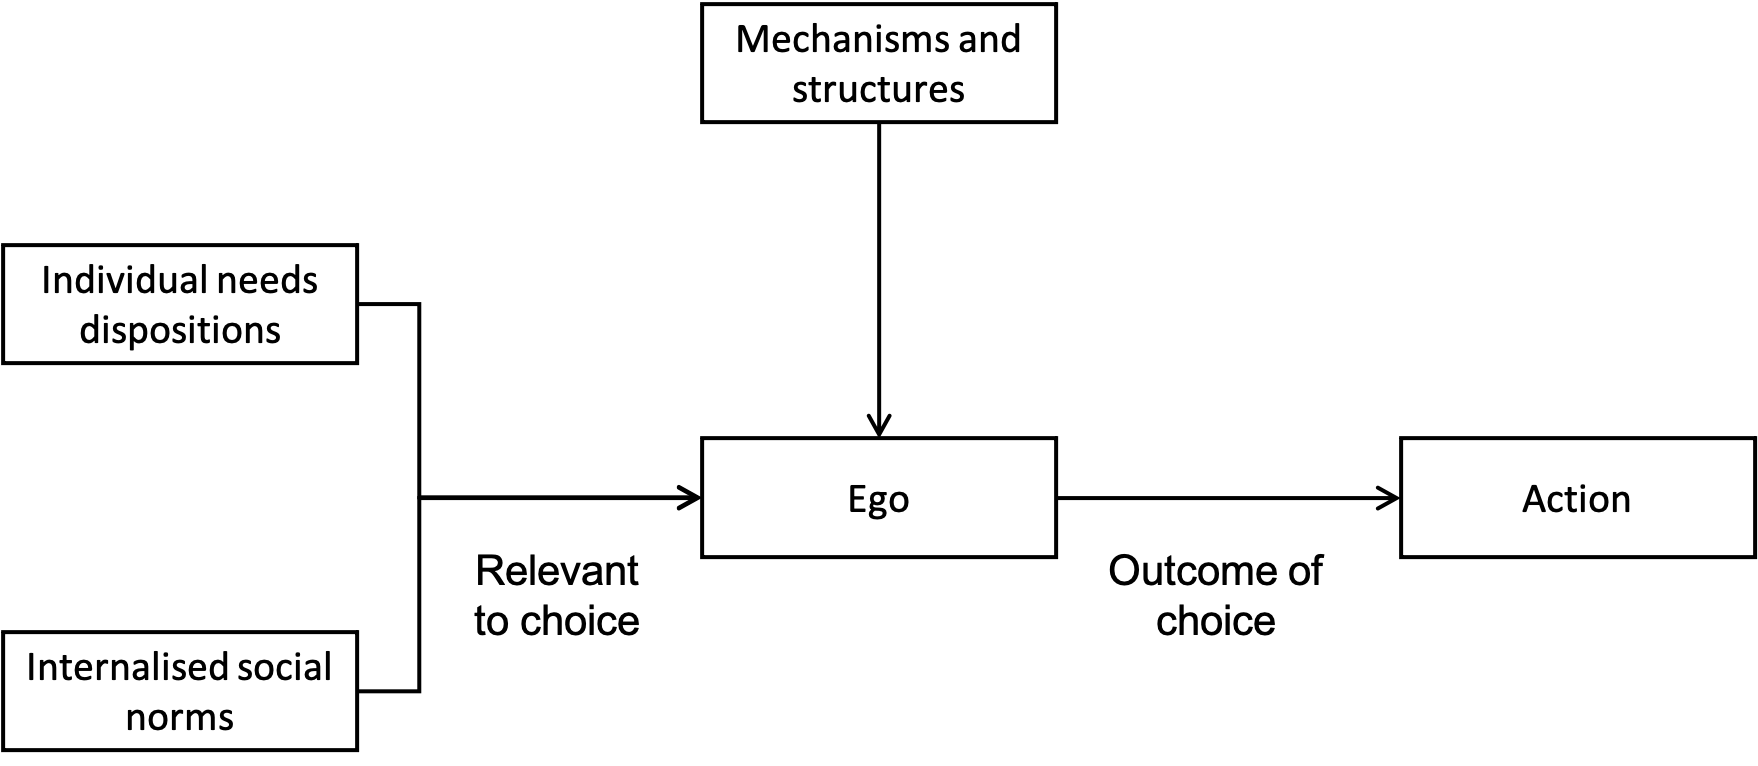
\includegraphics[width = \textwidth]{Images/agency_structure_loyal.png}
    \caption[]{Critical realist perspective of agency versus structure. Agency is about making intentional choices. Choices may be tempered by internalised social norms and social reality more broadly \citep{loyal2001agency}.}
    \label{fig:agency_structure3}
\end{figure}

This chapter begins by introducing the interviewees, referencing their role in their respective open innovation partnership, self-reported personal information, and position in their respective knowledge-sharing networks. It then presents the first- and second-cycle coding results for each case before concluding with a summary of the leading social mechanisms at play in each open innovation partnership.

\begin{table}[hbt!]
\centering
\small
\caption[]{Provisional codes derived from theoretical propositions.}
\label{tab:provcode3}
\resizebox{\textwidth}{!}{%
\begin{tabular}{ p{1cm} p{10cm} p{5cm} }
\toprule
Proposition & Statement & Provisional code \\ \midrule
\multirow{2}{=}{1a} & \multirow{2}{=}{Open innovation requires practitioners to connect across organisational and disciplinary boundaries so that they can transfer and apply their know-how and know-what in novel ways.} & Spanning real and perceived boundaries \\
 &  & Applying knowledge innovatively \\
\multirow{2}{=}{1b} & \multirow{2}{=}{Reducing cognitive distance between open innovation partners requires significant social  interaction to support learning and the application of knowledge in practice.} & Promoting a learning culture \\
 &  & Applying knowledge in practice \\
\multirow{2}{=}{2a} & \multirow{2}{=}{Successful open innovation requires deliberate brokerage actions that lead to network closure.} & Connecting people \\
 &  & Fostering collaboration \\
\multirow{2}{=}{3a} & \multirow{2}{=}{Formal structures inhibit tacit knowledge exchange in open innovation partnerships.} & Defining the rules of engagement \\
 &  & Encountering power structures \\
\multirow{3}{=}{3b} & \multirow{3}{=}{Innate needs and subjective norms moderate individual willingness to seek out or share tacit knowledge.} & Doing satisfying work \\
 &  & Expressing a particular worldview \\
 &  & Identifying with a distinct group \\
\multirow{1}{=}{4a} & Reciprocity and closure in tacit knowledge exchange networks indicate high levels of trust in open innovation partnerships. & Building trust relations \\
\multirow{2}{=}{4b} & \multirow{2}{=}{Who people choose to empower with their know-how depends on how much they trust the receiver to use their know-how in mutually beneficial ways.} & Empowering others \\
 &  & Protecting knowledge \\ \bottomrule
\end{tabular}%
}
\end{table}

\section{Participant information}

This study aimed to interview a cross-section of participants in terms of their partner affiliation and network position (i.e. central and peripheral actors in the knowledge provider networks). Not all the initially targeted participants were available to be interviewed. Participants that were available to be interviewed did reveal much about the social dynamics in each partnership. Table \ref{tab:interviewees} provides a breakdown of the participants interviewed in each case. Interviews ranged from 25 to 106 minutes in duration. The longer interviews usually involved participants with higher network centrality. Their privileged network position meant they were well-placed to provide useful information about knowledge exchanges. The sentiment analysis tool in \texttt{NVivo\texttrademark} was used to assess the general expressed by interviewees in their responses to semi-structured interview questions. Results of the sentiment analysis reveal what each interviewee feels about their particular partnership (Table \ref{tab:sentiment_case}).


\begin{table}[hbt!]
\centering
\caption[Details about each interview]{Details about each interview.}
\label{tab:interviewees}
\resizebox{\textwidth}{!}{%       
\begin{threeparttable}
\begin{tabular}{crrcrclccl}
\toprule

& \specialcell[t]{Network\\ID} &
\specialcell[t]{Employer} &
\specialcell[t]{Date of\\interview} &
\specialcell[t]{Duration\\(MM:SS)} &
\specialcell[t]{Interview\\mode} &
\specialcell[t]{Role} &
\specialcell[t]{Openness} &
\specialcell[t]{Network\\centrality} &
\specialcell[t]{Country} \\ 
\midrule
\multirow{6}{*}{\rotatebox[origin=c]{90}{Case 1} \rotatebox[origin=c]{90}{($n = 18$)}} 
& 1/1 & 1/1 & 18.12.2015 & 79:04 & F2F & General Manager & 0.44 & 31 & AU \\
& 3/1 & 1/1 & 26.04.2016 & 33:34 & F2F & Transport Manager & 0.61 & 18 & AU \\
& 8/1 & 2/1 & 11.03.2016 & 81:01 & F2F & Freight Company Owner & 0.78 & 12 & AU \\
& 10/1 & 3/1 & 07.03.2016 & 58:46 & F2F & International Sales Director & 0.72 & 2 & USA \\
& 15/1 & 7/1 & 25.02.2016 & 66:29 & F2F & Database Specialist & 0.72 & 11 & AU \\
& 16/1 & 7/1 & 07.09.2016 & 43:35 & F2F & Research Group Leader & 0.50 & 9 & AU \\ 
\midrule
\multirow{8}{*}{\rotatebox[origin=c]{90}{Case 2} \rotatebox[origin=c]{90}{($n = 25$)}} 
& 1/2 & 1/2 & 01.03.2016 & 59:21 & F2F & Dairy Farmer & 0.44 & 39 & AU \\
& 8/2 & 2/2 & 18.03.2016 & 70:02 & VL & Research Project Leader & 0.50 & 28 & AU \\
& 9/2 & 3/2 & 20.03.2016 & 106:10 & F2F & Farm System Specialist & 0.78 & 40 & NZ \\
& 10/2 & 4/2 & 18.03.2016 & 48:44 & VL & Technical Specialist & 0.61 & 18 & AU \\
& 11/2 & 5/2 & 04.03.2016 & 66:04 & F2F & Pasture Consultant & 0.78 & 11 & AU \\
& 15/2 & 7/2 & 03.11.2016 & 76:13 & F2F & Company Owner & 0.50 & 34 & AU \\
& 18/2 & 3/2 & 16.02.2016 & 69:02 & VL & Executive Manager & 0.44 & 26 & NZ \\ 
& 23/2 & 3/2 & 11.03.2016 & 24:53 & VL & Technical Specialist & 0.67 & 15 & SE \\ 
\midrule
\multirow{7}{*}{\rotatebox[origin=c]{90}{Case 3} \rotatebox[origin=c]{90}{($n = 40$)}} 
& 9/3 & 9/3 & 14.12.2016 & 61:35 & VL & Researcher & 0.61 & 18 & BR \\
& 10/3 & 10/3 & 16.03.2016 & 89:26 & F2F & Research Group Leader & 0.78 & 70 & AU \\
& 13/3 & 10/3 & 13.05.2016 & 35:42 & F2F & Project Coordinator & 0.72 & 35 & AU \\
& 16/3 & 10/3 & 12.09.2016 & 73:23 & F2F & Database Specialist & 0.89 & 23 & AU \\ 
& 22/3 & 10/3 & 19.09.2016 & 47:48 & VL & Executive Manager & 0.53 & 10 & AU \\ 
& 39/3 & 7/3 & 09.09.2016 & 27:14 & VL & Researcher & 0.61 & 10 & MX \\
& 41/3 & 1/3 & 07.10.2016 & 32:36 & VL & Database Specialist & 0.78 & 3 & NZ \\
\bottomrule
\end{tabular}
\begin{tablenotes}
% \footnotesize
\item $n$ refers to the number of respondents to the online survey.
\item F2F refers to face-to-face interviews, whereas VL refers to \texttt{Skype}\texttrademark\ interviews. 
\item Network centrality refers to number of incoming and outgoing social ties in the combined (tacit and explicit) knowledge network.
\item Country expressed in terms of ISO 3166 country code.
\end{tablenotes}
\end{threeparttable}
}
\end{table}

\begin{table}[hbt!]
\centering
\caption[Breakdown of sentiment]{Breakdown of sentiment by interviewee. The colours indicate the relative strength or dominance of a particular sentiment -- the redder the colour, the more dominant is the sentiment expressed by the interviewee.}
\label{tab:sentiment_case}
\begin{subtable}{1\textwidth}
\centering
\resizebox{\textwidth}{!}{%   
\begin{tabular}{r *{4}{c}}
\toprule
\multicolumn{1}{c}{}
Network ID & Very negative & Moderately negative & Moderately positive & Very positive \\ \midrule
1/1 & \gradientcell{24}{0}{50}{lime}{red}{90} & \gradientcell{26}{0}{50}{lime}{red}{90} & \gradientcell{46}{0}{50}{lime}{red}{90} & \gradientcell{13}{0}{50}{lime}{red}{90} \\
3/1 & \gradientcell{2}{0}{50}{lime}{red}{90} & \gradientcell{4}{0}{50}{lime}{red}{90} & \gradientcell{19}{0}{50}{lime}{red}{90} & \gradientcell{14}{0}{50}{lime}{red}{90} \\
8/1 & \gradientcell{16}{0}{50}{lime}{red}{90} & \gradientcell{23}{0}{50}{lime}{red}{90} & \gradientcell{37}{0}{50}{lime}{red}{90} & \gradientcell{12}{0}{50}{lime}{red}{90} \\
10/1 & \gradientcell{14}{0}{50}{lime}{red}{90} & \gradientcell{13}{0}{50}{lime}{red}{90} & \gradientcell{45}{0}{50}{lime}{red}{90} & \gradientcell{22}{0}{50}{lime}{red}{90} \\
15/1 & \gradientcell{11}{0}{50}{lime}{red}{90} & \gradientcell{18}{0}{50}{lime}{red}{90} & \gradientcell{35}{0}{50}{lime}{red}{90} & \gradientcell{10}{0}{50}{lime}{red}{90} \\
16/1 & \gradientcell{6}{0}{50}{lime}{red}{90} & \gradientcell{8}{0}{50}{lime}{red}{90} & \gradientcell{28}{0}{50}{lime}{red}{90} & \gradientcell{9}{0}{50}{lime}{red}{90} \\ \bottomrule
\end{tabular}
}%
\bigskip
\caption{Case 1}
\label{tab:sentiment_case_1}
\end{subtable}

\bigskip
\begin{subtable}{1\textwidth}
\centering
\resizebox{\textwidth}{!}{%   
\begin{tabular}{r *{4}{c}}
\toprule
\multicolumn{1}{c}{}
Network ID & Very negative & Moderately negative & Moderately positive & Very positive \\ \midrule
1/2 & \gradientcell{16}{0}{80}{lime}{red}{90} & \gradientcell{28}{0}{80}{lime}{red}{90} & \gradientcell{27}{0}{80}{lime}{red}{90} & \gradientcell{17}{0}{80}{lime}{red}{90} \\
8/2 & \gradientcell{11}{0}{80}{lime}{red}{90} & \gradientcell{17}{0}{80}{lime}{red}{90} & \gradientcell{33}{0}{80}{lime}{red}{90} & \gradientcell{23}{0}{80}{lime}{red}{90} \\
9/2 & \gradientcell{30}{0}{80}{lime}{red}{90} & \gradientcell{27}{0}{80}{lime}{red}{90} & \gradientcell{72}{0}{80}{lime}{red}{90} & \gradientcell{18}{0}{80}{lime}{red}{90} \\
10/2 & \gradientcell{6}{0}{80}{lime}{red}{90} & \gradientcell{6}{0}{80}{lime}{red}{90} & \gradientcell{42}{0}{80}{lime}{red}{90} & \gradientcell{11}{0}{80}{lime}{red}{90} \\
11/2 & \gradientcell{23}{0}{80}{lime}{red}{90} & \gradientcell{22}{0}{80}{lime}{red}{90} & \gradientcell{44}{0}{80}{lime}{red}{90} & \gradientcell{22}{0}{80}{lime}{red}{90} \\
15/2 & \gradientcell{25}{0}{80}{lime}{red}{90} & \gradientcell{39}{0}{80}{lime}{red}{90} & \gradientcell{41}{0}{80}{lime}{red}{90} & \gradientcell{22}{0}{80}{lime}{red}{90} \\
18/2 & \gradientcell{8}{0}{80}{lime}{red}{90} & \gradientcell{8}{0}{80}{lime}{red}{90} & \gradientcell{42}{0}{80}{lime}{red}{90} & \gradientcell{15}{0}{80}{lime}{red}{90} \\
23/2 & \gradientcell{2}{0}{80}{lime}{red}{90} & \gradientcell{3}{0}{80}{lime}{red}{90} & \gradientcell{10}{0}{80}{lime}{red}{90} & \gradientcell{5}{0}{80}{lime}{red}{90} \\ \bottomrule
\end{tabular}
}%
\bigskip
\caption{Case 2}
\label{tab:sentiment_case_2}
\end{subtable}

\bigskip
\begin{subtable}{1\textwidth}
\centering
\resizebox{\textwidth}{!}{%   
\begin{tabular}{r *{4}{c}}
\toprule
\multicolumn{1}{c}{}
Network id & Very negative & Moderately negative & Moderately positive & Very positive \\ \midrule
9/3 & \gradientcell{2}{0}{70}{lime}{red}{90} & \gradientcell{6}{0}{70}{lime}{red}{90} & \gradientcell{12}{0}{70}{lime}{red}{90} & \gradientcell{5}{0}{70}{lime}{red}{90} \\
10/3 & \gradientcell{15}{0}{70}{lime}{red}{90} & \gradientcell{24}{0}{70}{lime}{red}{90} & \gradientcell{66}{0}{70}{lime}{red}{90} & \gradientcell{28}{0}{70}{lime}{red}{90} \\
13/3 & \gradientcell{7}{0}{70}{lime}{red}{90} & \gradientcell{11}{0}{70}{lime}{red}{90} & \gradientcell{21}{0}{70}{lime}{red}{90} & \gradientcell{5}{0}{70}{lime}{red}{90} \\
16/3 & \gradientcell{14}{0}{70}{lime}{red}{90} & \gradientcell{19}{0}{70}{lime}{red}{90} & \gradientcell{47}{0}{70}{lime}{red}{90} & \gradientcell{22}{0}{70}{lime}{red}{90} \\
22/3 & \gradientcell{13}{0}{70}{lime}{red}{90} & \gradientcell{12}{0}{70}{lime}{red}{90} & \gradientcell{23}{0}{70}{lime}{red}{90} & \gradientcell{15}{0}{70}{lime}{red}{90} \\
39/3 & \gradientcell{1}{0}{70}{lime}{red}{90} & \gradientcell{4}{0}{70}{lime}{red}{90} & \gradientcell{2}{0}{70}{lime}{red}{90} & \gradientcell{2}{0}{70}{lime}{red}{90} \\
41/3 & \gradientcell{5}{0}{70}{lime}{red}{90} & \gradientcell{4}{0}{70}{lime}{red}{90} & \gradientcell{11}{0}{70}{lime}{red}{90} & \gradientcell{7}{0}{70}{lime}{red}{90} \\ \bottomrule
\end{tabular}
}%
\bigskip
\caption{Case 3}
\label{tab:sentiment_case_3}
\end{subtable}
\end{table}

\section{Case 1}

\subsection{Semi-structured interviews}

Six people were interviewed face-to-face in Case 1. Table \ref{tab:interviewees} contains important information about each interview. The interviewees included senior people from each partner organisation as well as participants working on specific project activities (Table \ref{tab:interviewees}). Due to scheduling conflicts, it took nine months to complete all the interviews. The length of the interviews ranged between 34 and 81 minutes (the average interview duration was 60 minutes). Table \ref{tab:sentiment_case_1} shows the overall sentiment expressed by each interviewee from Case 1. Most were positive about the open innovation partnership.

\subsection{Recap of network analysis}

The tacit knowledge provider network is quite sparse, suggesting that tacit knowledge is not widely shared in Case 1 (Figure \ref{fig:network_case_1}). The sparseness may be due to the fact that this case was at an early stage -- relationships were still developing. The ERGM results indicate people are more likely to share tacit knowledge with others in their immediate social group. Receivers of tacit knowledge tend to be trusted, open to experience, and autonomously motivated. Geography is a limiting factor for tacit knowledge exchanges. Explicit knowledge mostly flows to a few central actors who are likely to be from the same organisation. Providers of explicit knowledge tend to have been in their jobs for some time (Table \ref{tab:ergm_1}). \medskip

The ERGM analysis of broker roles shows that the representative broker role is over-represented in the tacit knowledge provider network. The liaison broker role is over-represented in the explicit knowledge provider network (Table \ref{tab:ergm_3}). Whereas the modelling assesses whether broker roles are under or over-represented for all possible two-path configurations, the raw broker counts presented in Figure \ref{fig:gf_c1} show which participant is the dominant broker in each network. For example, Participant 1/1 stands out as the dominant broker, acting primarily in a liaison and gatekeeper role in the explicit knowledge network and to a lesser extent in a representative and internal coordinator role in the tacit knowledge network. Responses to semi-structured interview questions help us understand how Participant 1/1 influenced knowledge flows in both networks.  

\begin{figure}[hbt!]
\centering
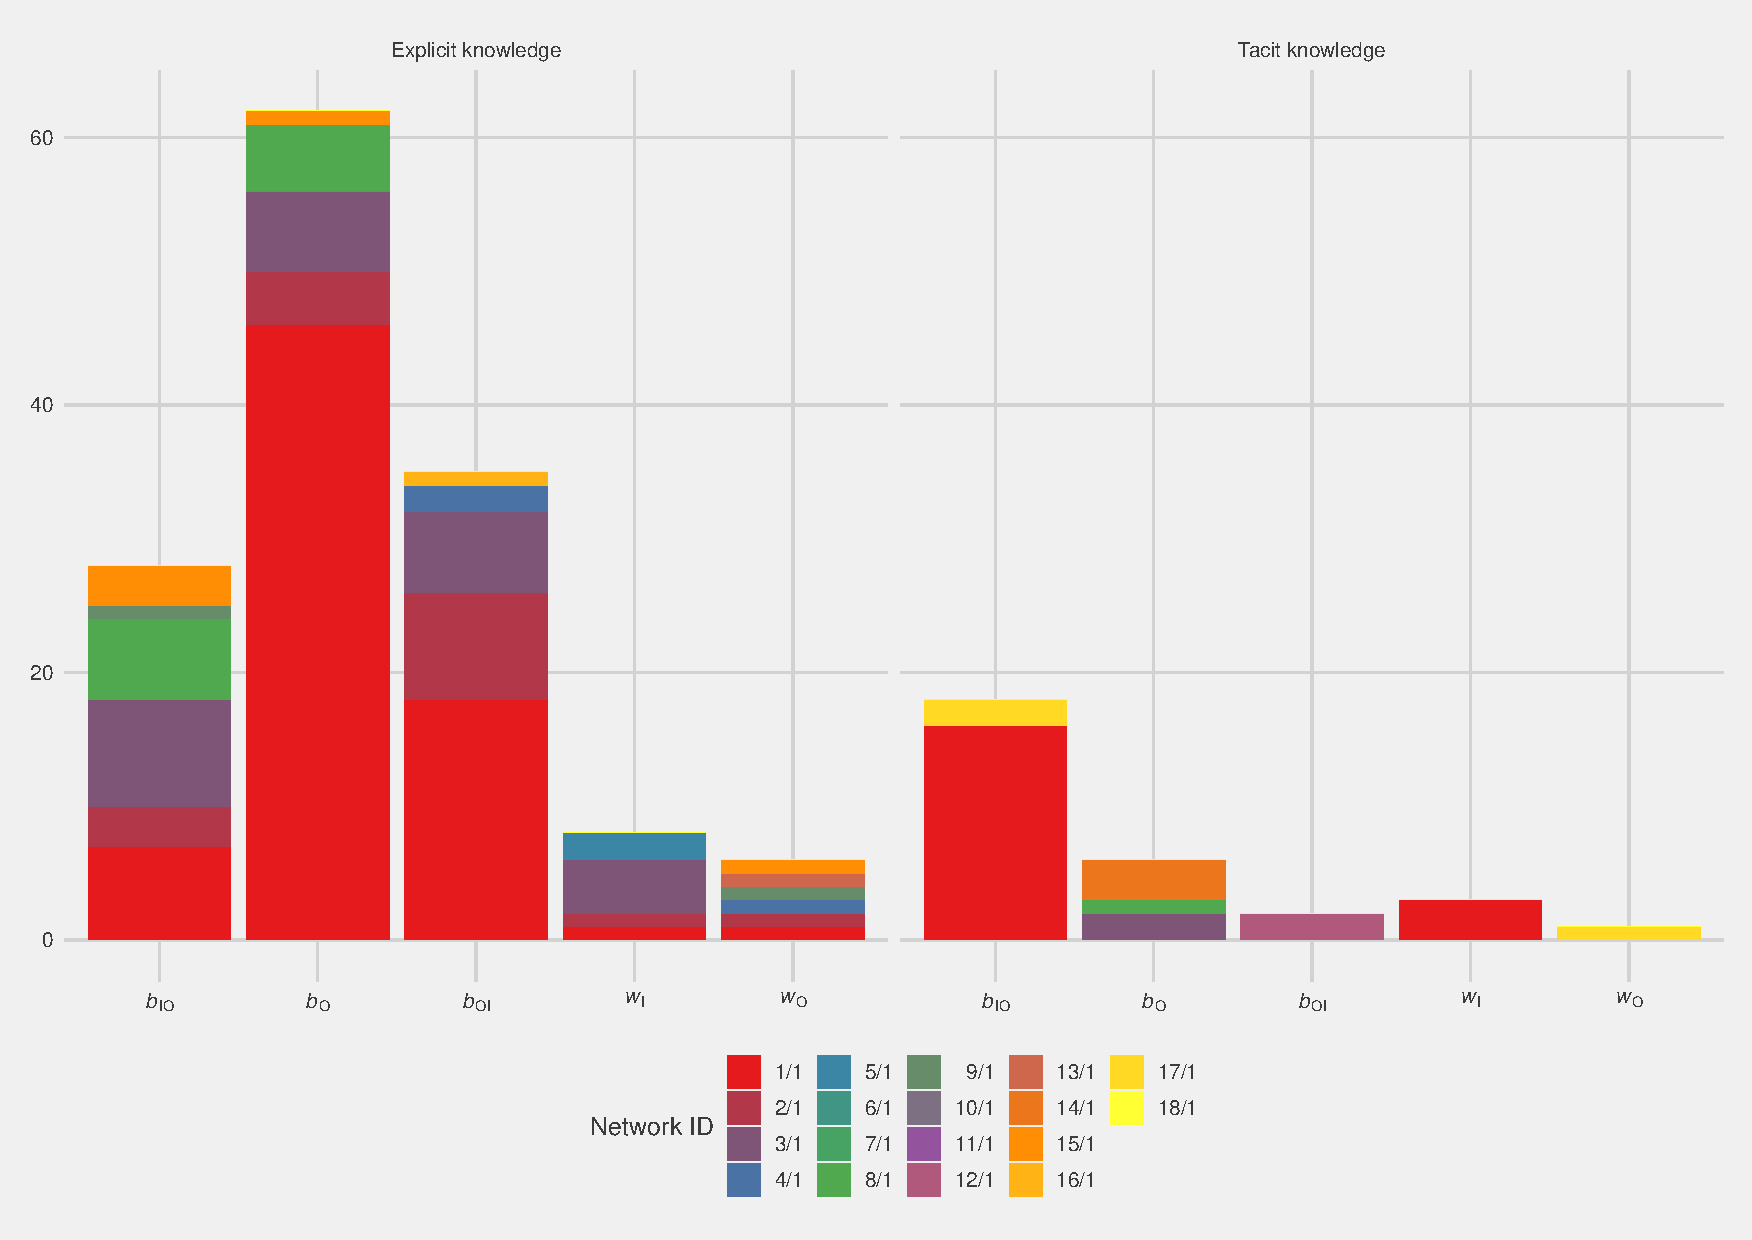
\includegraphics[width = \textwidth]{Images/gf_case1.pdf}
\caption[Raw broker role counts by participant in Case 1]{Raw broker role counts by participant in Case 1. Counts were generated by the \texttt{sna} package in \texttt{R} \citep{butts2016sna}. Note $w_I$ = internal coordinator role, $b_O$ = liaison role, $b_{OI}$ = gatekeeper role, $b_{IO}$ = representative role, and $w_O$ = itinerant broker role. Participant 1/1 stands out as a dominant broker.}
\label{fig:gf_c1}
\end{figure}

\subsection{Analysis of interview transcripts}

The qualitative analysis sheds light on the factors affecting the dynamic interaction between agency and structure. Coding involves the interpretive analysis of diverse narratives stemming from responses to open-ended questions. Table \ref{tab:case_1_codes} breaks down the most frequently cited concerns of interviewees in each category (innate needs, internalised social norms, social mechanisms or structures, and actions). The category codes refer to the main elements of \citeauthor{loyal2001agency}'s \citeyearpar{loyal2001agency} agency mode (Figure \ref{fig:agency_structure3}). \medskip

With respect to innate needs and subjective norms, the desire to perform interesting and meaningful work was an important motivator for most interviewees. However, the sharing of know-how appears to be tempered by participants worried about potential changes to their role and beliefs about the absorptive capacity of others. Key mechanisms and structures moderating tacit knowledge exchanges include the need to have good relations to facilitate open and honest discussions, swift trust, difficulty accessing knowledgeable people and poor communication. Actions revolved around broadening understanding to improve practices, tapping external expertise, and brokering (or restricting) knowledge exchanges. 

\begin{sidewaystable}[hbtp]
\centering
\caption{Most frequently referenced codes in each category: Case 1.}
\label{tab:case_1_codes}
\resizebox{\textwidth}{!}{%
\begin{tabular}{lllc}
\toprule
Category code & Provisional code & Detailed code & References \\ \midrule
Innate needs & Doing satisfying work & Performing meaningful work & 6 \\
Innate needs & Seeking autonomy & Becoming more competent & 1 \\
Internalised social norms & Expressing a particular worldview & Maintaining a narrow perspective & 6 \\
Internalised social norms & Expressing a particular worldview & Demonstrating a superior attitude & 4 \\
Internalised social norms & Expressing a particular worldview & Navigating change & 3 \\
Internalised social norms & Identifying with a distinct group & Being absolutely committed to the partnership & 2 \\
Mechanisms \& structures & Building trust relations & Investing in relationships & 13 \\
Mechanisms \& structures & Building trust relations & Having open and honest discussions & 11 \\
Mechanisms \& structures & Building trust relations & Demonstrating swift trust & 9 \\
Mechanisms \& structures & Spanning real and perceived boundaries & Gaining access to key people & 9 \\
Mechanisms \& structures & Encountering power structures & Dealing with large organisations & 8 \\
Action & Applying knowledge in practice & Improving practices & 30 \\
Action & Connecting people & Practising liaison brokerage & 17 \\
Action & Promoting a learning culture & Gaining a broader understanding & 16 \\
Action & Promoting a learning culture & Tapping external expertise & 15 \\
Action & Connecting people & Gatekeeping & 11 \\ \bottomrule
\end{tabular}%
}
\end{sidewaystable}

\subsubsection{Innate needs}

According to the theory of self-determination, people are primarily motivated by an innate need for autonomy, competence, and relatedness \citep{deci1989self}. Autonomy refers to an individual's ability to have control over their actions and autonomy, while autonomy support refers to an individual's perception of their social environment and the extent to which it allows them freedom of choice and acknowledges their opinion \citep{sweet2012testing}. Competence is about feeling effective in one's ongoing interactions with the social environment and experiencing opportunities to exercise and express one's capacities \citep{vansteenkiste2020basic}, and relatedness refers to the desire to feel connected to others in a given context \citep{deci2001need}. Satisfaction of these three psychological needs leads to greater levels of self-determined motivation \citep{sweet2012testing}. The qualitative analysis reveals that participants are motivated either by a desire to perform meaningful work, do something interesting, or become or feel more competent. In other words, the need for autonomy and competence are critical motivators for participants in Case 1. Regarding meaningful work, the university participants interpreted it as:

\begin{quote}
\small
\enquote{Being seen to be involved in [a particular region] with a major producer out there doing things, hopefully producing something that is meaningful.} \\
\rightline{\rm --- Participant 15/1}
\end{quote}

\begin{quote}
\small
\enquote{I think for any researcher, if you think the work that you do will actually be utilised and you can see evidence of it, well that’s a pretty big kick.} \\
\rightline{\rm --- Participant 16/1}
\end{quote}

The owner of the freight company indicated that being invited to participate in the cold-chain initiative was quite meaningful for him and his company:

\begin{quote}
\small
\enquote{[The green leafy vegetable grower] getting us involved as a transport operator helping them, is what I enjoy.} \\
\rightline{\rm --- Participant 8/1}
\end{quote}

The leader of the university research group could see that the owner of the freight company was keen to be involved in the cold-chain initiative and was happy to provide information to the university researchers. Much of this was driven by the owner's keen interest in cold-chain logistics:

\begin{quote}
\small
\enquote{the guy who we spoke to was the owner [of the freight company] -- he was really interested. So I think what happened was that there was an interest level that was really driving it more than anything else.} \\
\rightline{\rm --- Participant 16/1}
\end{quote}

The manager of freight logistics at the leafy vegetable grower also showed a keen interest in the research being done by the university researchers:

\begin{quote}
\small
\enquote{It'll be interesting to find out what their thoughts are and things that they think we can improve on and different things like that for sure.} \\
\rightline{\rm --- Participant 3/1}
\end{quote}

One of the university researchers felt good about himself for creating a software tool to ingest and report on temperature data collected by sensors strategically placed in a fully laden refrigerated truck compartment:

\begin{quote}
\small
\enquote{I probably actually have enjoyed the data analysis tool the most, because we had say 150 sensors in there and I wrote the data loading script and the database to store the data in and then just seeing all the data and seeing that it made sense, I think, was probably pretty enjoyable, that was a good, a good outcome for me.} \\
\rightline{\rm --- Participant 3/1}
\end{quote}

For many participants, innate needs are evident in their strong desire to do work that is both meaningful and interesting. Put differently, there was evidence of innate needs relating to doing meaningful work across participants. 

\subsubsection{Internalised social norms}

The qualitative analysis reveals that knowledge-sharing behaviour might be influenced by people with narrow perspectives, a condescending or superior attitude, and anxiety around affecting change. The owner of the freight company is keenly interested in anything to do with the cold chain:

\begin{quote}
\small
\enquote{I've always been very, very conscious, and maybe fanatical about having facilities that can keep product cold ... so with that you learn about air flow, and cold air and what's best and what’s not best, and you take advice from people who make the fridges, and who make the vans, and who talk about insulation ... for the last 22 or 23 years of my life I've [been a student of] refrigerated transport.} \\
\rightline{\rm --- Participant 8/1}
\end{quote}

However, he prefers to keep a narrow focus on what his company does best, i.e. transporting perishable goods. Although the freight company owner can see how [the leafy vegetable grower]'s and the supermarket chains' processes can impact his operation negatively, he feels these are beyond his control. All his company can do is get temperature sensitive goods to customers as quickly as possible:  

\begin{quote}
\small
\enquote{We need to concentrate, our business needs to concentrate on what we do, which is to be a refrigerated transport supplier ... that's what we try and instil in all our customers, is to move the freight. That's the bottom line. People want their product to be moved. [The green leafy vegetable grower] want[s] the best financial result, and the best delivery result in the least amount of time.} \\
\rightline{\rm --- Participant 8/1}
\end{quote}

The general manager in charge of supply chain and procurement at the leafy vegetable grower thinks the freight companies are too focused on providing cold air and not giving enough attention to how airflow impacts products in transit:

\begin{quote}
\small
\enquote{The freight companies ... firmly believe that if I put the set point of my refrigerator on the van at two degrees, and the readout throughout the journey says two degrees, I've done my job. And that's still open to discussion ... one thing that we've discovered is that how the product's loaded definitely has an impact on how it's cooled during a journey, because airflow, if air doesn't get to the product then it doesn't get cooled.} \\
\rightline{\rm --- Participant 1/1}
\end{quote}

It seems this narrow focus led both the leafy vegetable grower and university researchers to think that freight companies are not particularly interested in the research being undertaken. Either that, or they doubt the freight companies have the absorptive capacity to understand thermodynamics:

\begin{quote}
\small
\enquote{I don't think they ever look at it scientifically, I think they just look at it very broadly, and that's as far as they go ... what they will say is \enquote{explain it to me simply, don't come to me with a whole bunch of scientific jargon and things, just say to me, well the reason it doesn't work is because the gap between the top of the van and the pallets is too narrow and your airflow doesn't work, and that's why things don't get cooled at the back of the van at all, and never will}.} \\
\rightline{\rm --- Participant 1/1}
\end{quote}

\begin{quote}
\small
\enquote{If you were talking to [the freight company] yeah, you don't want to start talking about thermal masses and all that sort of stuff.} \\
\rightline{\rm --- Participant 15/1}
\end{quote}

Not wanting to explain things in detail appeared to deny the freight companies the opportunity to learn more about thermodynamics, despite the strong desire of the owner of the main freight company to learn about and implement good cold-chain practices. The general manager also felt his organisation suffered from a silo mentality that affected internal sharing of knowledge and/or ideas: 

\begin{quote}
\small
\enquote{There’s this silo mentality in the business that we need to break, and I think once you've broken that then you'll... then there will be a lot more idea sharing, and a lot more new things that we want to do and want to try out.} \\
\rightline{\rm --- Participant 1/1}
\end{quote}

This silo mentality is evident in the attitude of his transport manager who prefers to focus on his immediate area of responsibility: 

\begin{quote}
\small
\enquote{Like I said, I just basically focus on my specific job at hand, and don't really look outside the box too much, whereas it probably would be handy, like you said, to look outside the box, and see what we can actually bring to the company to improve the different sides of the company, like the freight and different things.} \\
\rightline{\rm --- Participant 3/1}
\end{quote}

The general manager was worried that the cold-chain initiative would not deliver expected outcomes. Although he wants to reduce supermarket rejections, he was also keen to strengthen relations with his supermarket chain customers by increasing the shelf-life of his company's leafy vegetable products. He mentioned that his company does not have ongoing supply contracts with the major supermarket chains. Providing good quality products to major supermarket customers helps secure ongoing business. Extending the shelf-life of products also helps supermarkets reduce food waste. They will be more inclined to support businesses that create additional value for them. The general manager was relying on the cooperation of people within his organisation, the refrigerated freight companies, and supermarket customers to deliver outcomes and was concerned that people would not be willing to change their ways:

\begin{quote}
\small
\enquote{I think once you dig deeper into the process and try and establish now where the root cause of a warm bag might be, or whatever it might be, you see if you don't have the right people in there to help you, you’re not going to get very far, because they don't want... they like things the way they are, they don't want someone to come along and say \enquote{Hey, guess what, from tomorrow you've got to shake the bag three or four time before you put it in the box, because by shaking it you'll improve the airflow through the product, and the temperature settles down more, and you don't get hot-spots} and all that sort of stuff.} \\
\rightline{\rm --- Participant 1/1}
\end{quote}

In terms of subjective norms, a reluctance to see the bigger picture and unwillingness to change practices might have affected knowledge exchanges in the cold-chain initiative. Some participants appeared to doubt the absorptive capacity of the freight companies around thermodynamic modelling and product performance. The extent to which this doubt is due to freight companies being narrowly focused on supplying cold air or the reluctance of university-educated participants to make an effort to share knowledge and understanding is not clear. It seems that perceived rather than actual absorptive capacity is an issue here.

\subsubsection{Social mechanisms \& structures}

Being able to have open discussions, build quality relationships, access busy people, trusting others from the outset, and communicate effectively appear to be the main social mechanisms affecting knowledge exchanges in this case. One indicator of trust is the ability to have open and honest discussions. Not only do open and honest discussions help build trust, trust also enables open and honest discussions:

\begin{quote}
\small
\enquote{I think that over time you can build up trust, and then you can share your knowledge and different things like that.} \\
\rightline{\rm --- Participant 3/1}
\end{quote}

\begin{quote}
\small
\enquote{The amount of information shared is less if I do not trust the person and trust, in my opinion, can be built up over time.} \\
\rightline{\rm --- Participant 10/1}
\end{quote}

One university researcher made an interesting point about explicit and tacit knowledge sharing that may have profound implications for relationship and trust building:

\begin{quote}
\small
\enquote{Explicit knowledge sharing comes after you've built the relationships that enable tacit knowledge [exchange].} \\
\rightline{\rm --- Participant 15/1}
\end{quote}

He is suggesting that informal structures that support tacit knowledge sharing are essential for explicit knowledge exchange. Yet, it has been found that employees are not always aware of their tacit knowledge \citep{polanyi1966tacit, horvath2000working}. Companies tend to discount the tacit knowledge embodied in employees \citep{mcadam2007exploring}. The manager of freight logistics at the leafy vegetable grower made this remark about tacit knowledge being discounted:

\begin{quote}
\small
\enquote{Whereas I might think it's very important for someone to share this knowledge so we can actually look at improving different things, but they may not think it's that important.} \\
\rightline{\rm --- Participant 3/1}
\end{quote}

This remark suggests that participants may withhold tacit knowledge because they do not consider their know-how is worth sharing. According to the owner of the main freight company, trust allows one to engage in difficult conversations that help surface problems and bring these into sharper focus. He believes it is easier to resolve problems this way:   

\begin{quote}
\small
\enquote{We can have those conversations, because you need to, it's healthy to be able to debate the issue ... The fact that we have tension, and that we create tension, is because we trust each other ... because tension is created by a cock up, if you want to put it that way. So what's the best way to fix that problem? Be innovative, or fix it.} \\
\rightline{\rm --- Participant 8/1}
\end{quote}

Swift trust did feature in this open innovation partnership. The general manager driving the cold-chain initiative did not know the university researchers well but assumed they were competent and knew what they were doing:

\begin{quote}
\small
\enquote{when [the head of the university team] came along and introduced me to his team, I do form an opinion on who I'm working with by ... you know, and I spend a bit of time talking to them and that sort of stuff. So, but I suppose, too, part of the whole, you know part of this whole collaboration thing with the university is that I suppose you have to trust the people that you’re going to work with ... I'm trusting them that they know what they're doing and why they're doing it, and what they're going to be able to get out of it at the end of it.} \\
\rightline{\rm --- Participant 1/1}
\end{quote}
 
However, his other comments suggested that others were less capable of sharing knowledge and that his role was to facilitate such exchanges. Another obstacle to knowledge sharing was finding time to engage with busy people. The university researchers initially struggled to gain access to people with relevant know-how in the leafy vegetable growing operation:   

\begin{quote}
\small
\enquote{Initially, trying to get contact with [the green leafy vegetable grower] was challenging at times, as you'd understand when you're trying to do research with a company because they've got operational imperatives that they need to manage and they have day-to-day crises that they need to manage.} \\
\rightline{\rm --- Participant 16/1}
\end{quote}

However, as relationships developed and research credibility was established, it became easier for the university researchers to connect with personnel at the leafy vegetable growing operation:

\begin{quote}
\small
\enquote{The link between us and the university is getting stronger as I get to know the guys more, and get to talk to them more, and find out what they're doing and why they're doing it, that is starting to become a fairly strong relationship there ... I'm trusting them that they know what they’re doing and why they’re doing it, and what they're going to be able to get out of it at the end of it.} \\
\rightline{\rm --- Participant 1/1}
\end{quote}

\begin{quote}
\small
\enquote{What I really noticed was as we started to go through the process and building up credibility, [the leafy vegetable grower] could see there were potential outcomes here, then they were ringing us more.} \\
\rightline{\rm --- Participant 16/1}
\end{quote}

Yet it appears the general manager was not particularly open himself, withholding knowledge from others. His transport manager, for example, expresses some frustration at not being kept in the loop about the results of the experimental trials conducted by the university researchers:

\begin{quote}
\small
\enquote{I haven't honestly seen a real lot of the results from the different university trials and things like that. So from my point of view it probably hasn't been as open as what it could be ... I'm not quite sure why the knowledge hasn't been passed down, or whether it's been passed to other people and not to me. I don't know.} \\
\rightline{\rm --- Participant 3/1}
\end{quote}

Given the transport manager is a central actor in both the tacit and explicit knowledge provider networks (Figure \ref{fig:network_case_1}), leaving him out of the communication loop does appear restrictive. The experimental trials do relate to the transport manager's area of responsibility. Not keeping him abreast of developments has caused some resentment and may explain why he was not particularly forthcoming in his interview. \medskip

The primary mechanism or structure moderating tacit knowledge exchanges seems to be the presence of trust. Trust promotes more open and transparent communication. The importance of trust is also evident in the ERGM results, where we see significant overlap between tacit knowledge sharing and cognition-based trust ties. Interesting insights from the qualitative analysis include the importance of informal structures for tacit and explicit knowledge sharing and discounting of tacit knowledge. Perceptions about the absorptive capacity of others have resulted in selective communication (e.g. the general manager did not think his transport manager would understand what the university researchers were up to).

\subsubsection{Actions}

Improving practices, connecting partners, engaging in learning, and gatekeeping are actions that stand out in Case 1. The cold-chain initiative is all about prolonging the shelf-life of leafy vegetable products through improved cold-chain practices:

\begin{quote}
\small
\enquote{It'll allow us to ... work on better methods to transport our product, and get to a point where we know that when we send our product that we've packed it and palletised it, and loaded it into the vans in the best possible manner, which will give us the best possible outcome throughout the journey.} \\
\rightline{\rm --- Participant 1/1}
\end{quote}

The freight company owner was pleased the leafy vegetable grower was tapping into their refrigerated transport expertise. He described one instance where his company advised the grower on how best to set up their loading docks: 

\begin{quote}
\small
\enquote{so we go down to their facility, have a look around, there's your floor. There's your slope. This is where you should put your docks. You need 37 metres for a normal truck to be able to back. And then you need to have a little bit more in case the driver [misjudges things], we step it out. These timing docks with the air bags and the ramp is fine. You need it to be 1.2 metres high, because that’s an average height of your van. So you need to dig this out, or put concrete or gravel down. No, no, you need to do concrete, because you've got the trucks that need to be secure. You can't have them sinking, you'll be filling in potholes all the time. You'll need to spend money on concrete. You need to do this, you need to do that. You need to have doors that go up and down. You need to have doors that can open, allow the vans to open. So that when you put your four or five pallets in, you can close the doors and keep the temperature in the van.} \\
\rightline{\rm --- Participant 8/1}
\end{quote}

The general manager never mentioned this advice in his interview. He did not acknowledge the input of the freight company at all in his interview, rather he complained about their narrow view of refrigerated transport. The general manager saw more value in soliciting input from the university researchers. He happily facilitated interaction between the university and other parts of his organisation (operating in a liaison broker role):

\begin{quote}
\small
\enquote{And I also put them in touch with people on the processing side and the farm side, so they could, if they wanted to ask any further questions they could. Especially for processing, one of the key things is around product shelf-life, and you know what impacts product shelf-life. So we've got a couple of people here who do data shelf-life testing, and they have a fairly strong view on what impacts shelf-life, you know, and after all like our product gets washed and dried, and then put in a bag, so you've got this like micro-environment there, and nobody really knows what happens in there, and I felt that they needed to understand that.} \\
\rightline{\rm --- Participant 1/1}
\end{quote}

He also saw himself as an interpreter, helping the freight companies understand understand the experiments the university researchers were attempting: 

\begin{quote}
\small
\enquote{I believe I'm pretty good [at just] explaining something that is slightly more complicated in a much simpler fashion, so and relate it to more day to day stuff. So the way I interact with the [university] guys when they're here, and the way I interact with the freight companies, and the people that work there, completely different.} \\
\rightline{\rm --- Participant 1/1}
\end{quote}

It could be argued that the general manager was boosting the absorptive capacity of the freight companies in his role as interpreter. It does suggest that he also harboured doubts about the absorptive capacity of the freight companies. Given that the freight company owner was hungry for knowledge, such doubt may be unfounded. The general manager was also a gatekeeper, not allowing university researchers to engage freight providers directly. He argued that allowing the university researchers too much independence would be pretty disruptive: 

\begin{quote}
\small
\enquote{I said to the [university] that if they need to spend some time with [the freight company] and use some of their equipment, that I'm the person who paves the way for them to go there and do it, rather than them doing it, because I'm the one who sort of spoke to the service providers and we’re all in agreement that there's something in it for all of us. So, but it's really it just needs one person to co-ordinate it, because if I had three or four people ringing up [the freight company] saying \enquote{Oh, we want to do this, we want to do that}, it would be quite messy.} \\
\rightline{\rm --- Participant 1/1}
\end{quote}

\begin{quote}
\small
\enquote{But in terms of [the general manager], obviously [he] is the person that you go to pretty much.} \\
\rightline{\rm --- Participant 15/1}
\end{quote}

Although the general manager does not appear to want the university researchers to complicate his relationships with freight companies, his motive for limiting access to the freight companies may be more about protecting his employer's commercial interests. The university researchers may inadvertently leak commercially sensitive information to the freight companies:

\begin{quote}
\small
\enquote{We've said to [the general manager] about doing a presentation to the two different trucking companies, and he said he'll let us know when he wants to do that. Because there’s a lot of commercial confidence and information there ...} \\
\rightline{\rm --- Participant 16/1}
\end{quote}

Despite the gatekeeping and doubts about the absorptive capacity of the freight companies, most participants were open to learning. Certainly, the freight company owner was keen understand what the university researchers had discovered so he could implement any necessary changes:

\begin{quote}
\small
\enquote{I'd love to know what actually happens when it gets made or packed, and what actually happens when it comes out as a report. We're big enough to stand up and say, OK, what problems have we got here, and how can we fix those up.} \\
\rightline{\rm --- Participant 8/1}
\end{quote}

Both the wireless temperature sensor provider and university researchers appreciated being exposed to the leafy vegetables grower's operation. This exposure allowed them to observe and better understand their in-house cold-chain practices:

\begin{quote}
\small
\enquote{What I enjoy, at least about my job and this collaboration is that the company, including [the general manager], is letting me into an in-depth process so we can truly tailor a solution to them.} \\
\rightline{\rm --- Participant 10/1}
\end{quote}

\begin{quote}
\small
\enquote{The best part of it was when they took us for the tour. So going through all their operations from start to finish. That helped to provide the context and the realism for us. So we could actually see what was happening and their rationale for doing certain things.} \\
\rightline{\rm --- Participant 16/1}
\end{quote}

The general manager recognises his organisation does not have the capacity to conduct basic research. He embraced inbound open innovation as a way to improve his organisation's cold-chain practices. Open innovation allows him to bring external expertise to bear on his innovation challenge:

\begin{quote}
\small
\enquote{The amount of effort that's needed to – and knowledge as well – the amount of effort and time required is something that our business does not have the time for, nor the manpower. And also, you know, the scientific knowledge, we don't have that either, so for me it's really important to collaborate with someone who has the means of looking at the problem, setting out experiments, and conduct experiments, to be able to identify what the, you know what the key factors are that might affect product temperature during transit.} \\
\rightline{\rm --- Participant 1/1}
\end{quote}

Actions are dominated by efforts to improve cold-chain practices. Efforts include tapping external expertise to gain a deeper understanding of airflow within refrigerated truck compartments. The ERGM analysis shows that the representative broker role is over-represented in the tacit knowledge provider network, which indicates that partners are happy to share tacit knowledge with others. However, it appears that the emergence of informal structures critical for tacit knowledge sharing is influenced by brokerage practices. The general manager seems happy to connect university researchers with personnel inside his organisation but is less inclined to allow the researchers to engage directly with with his freight and sensor technology providers. His actions appear to limit tacit knowledge exchanges, which might explain why the tacit knowledge network is so sparse in Case 1.

\subsection{Case synopsis}

Although the tacit knowledge network in Case 1 is sparse, the survey results show that most participants have a high level of autonomous motivation. The network analysis indicates that autonomously motivated people are more likely to seek out tacit knowledge, but that geography is a limiting factor. The general manager mentioned that working across different time zones challenged communication. Likewise, the sales director from the micro-sensor technology provider indicated it was important to travel from the USA to see things firsthand. It is clear from the qualitative analysis that the level of openness varies. Participants do not enjoy equal access to critical information and know-how. Perceptions about trustworthiness and the absorptive capacity of others are the main factors affecting the level of openness. The refrigerated freight companies have valuable know-how borne from many years of experience. Not allowing the university researchers agency to work directly with the freight companies appeared to limit tacit knowledge exchanges, which may explain why the tacit knowledge network is so sparse. Failure to engage more directly with the freight companies and selective communications, are considered the main risk factors in this open innovation partnership.

\section{Case 2}

\subsection{Semi-structured interviews}

Eight people were interviewed over 10 months in Case 2. Interviews lasted between 25 minutes and 106 minutes (the average interview duration was 65 minutes). Looking at the overall sentiment expressed by interviewees (Table \ref{tab:sentiment_case_2}), apart from the dairy farmer (Participant 1/2) and the local agent for the milking technology company (Participant 15/2), interviewees were mostly positive about the open innovation partnership. The main representative for the milking technology company (Participant 9/2) stands out as the most positive interviewee, which may partly explain why he was so effective at managing tensions and difficult relationships in the partnership.

\subsection{Recap of the network analysis}

Figure \ref{fig:network_case_2} indicates that tacit knowledge plays a key role in Case 2. The ERGM analysis reveals brokerage is under-represented and closure over-represented in the tacit knowledge provider network, a sign of strong collaboration (Table \ref{tab:ergm_1}). Participants with substantial work experience are the primary sources of tacit knowledge. As with Case 1, receivers of tacit knowledge tend to be autonomously motivated and are expected to be predisposed to learning. While tacit knowledge tends to circulate more among work colleagues, it is less likely to be shared with supervisors. Participants are more likely to share both their tacit and explicit knowledge with trusted others. \medskip

Figure \ref{fig:gf_c2} shows the breakdown of broker role counts in Case 2. The liaison broker role dominates both the explicit and tacit knowledge networks. What is particularly interesting is that broker roles are spread across many participants, interpreted as another sign of strong collaboration. Although the liaison broker role is dominant, the modelling of the tacit knowledge network shows that for all possible broker configurations, the liaison, gatekeeper, and representative roles are significantly under-represented (Table \ref{tab:ergm_2}). This under-representation is consistent with the significant and negative multiple connectivity (alternating two-path) effect seen in the other modelling results.

\begin{figure}[hbt!]
\centering
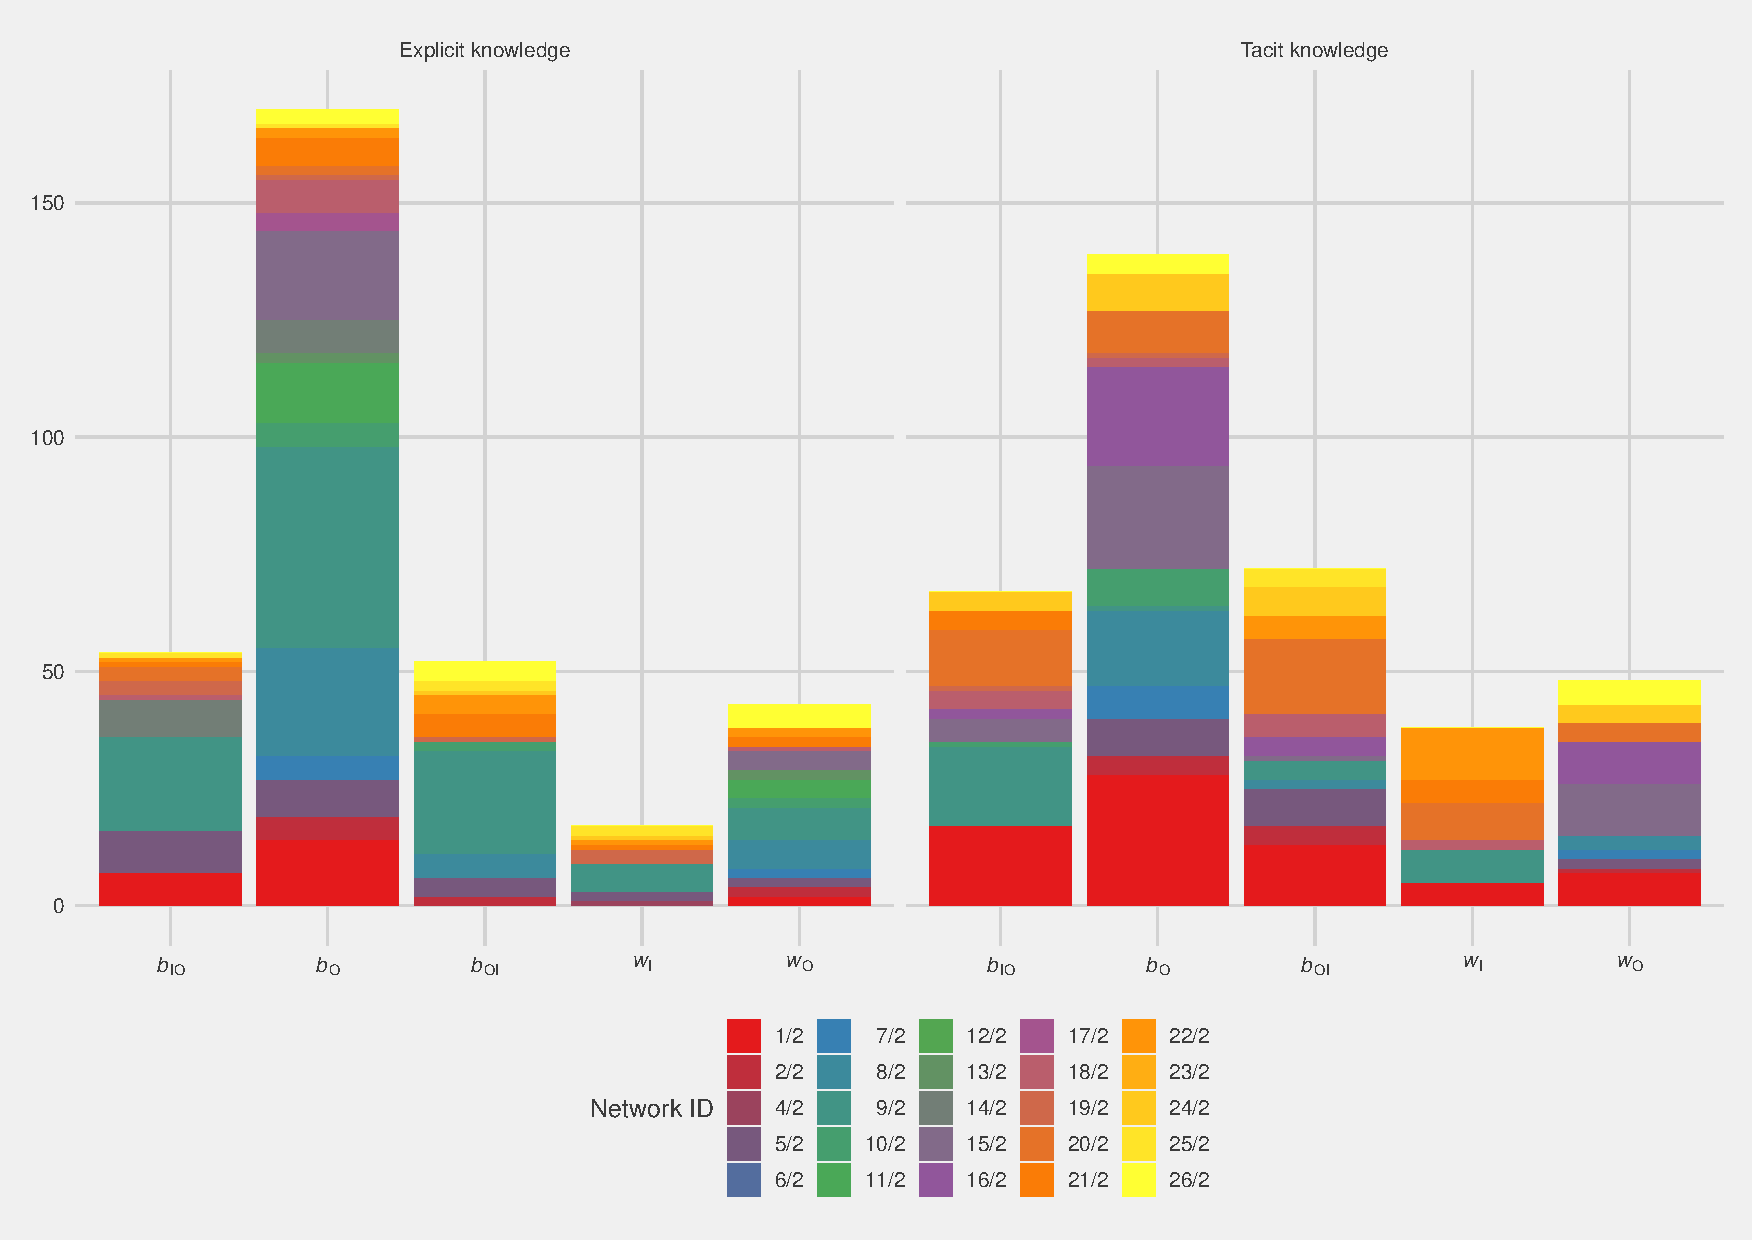
\includegraphics[width = \textwidth]{Images/gf_case2.pdf}
\caption[Raw broker role counts by participant in Case 2]{Raw broker role counts by participant in Case 2. Counts were generated by the \texttt{sna} package in \texttt{R} \citep{butts2016sna}. Note $w_I$ = internal coordinator role, $b_O$ = liaison role, $b_{OI}$ = gatekeeper role, $b_{IO}$ = representative role, and $w_O$ = itinerant broker role.}
\label{fig:gf_c2}
\end{figure}

\subsection{Analysis of interview transcripts}

Table \ref{tab:case_2_codes} lists the most frequently cited codes in each category. We see that the desire to become more competent, perform meaningful work, and connect with others dominates innate needs. Regarding internalised social norms, everybody showed a high level of personal commitment to the partnership. Some remarks were made about being over-analytical and holding superior attitudes. Mechanisms and structures moderating tacit knowledge exchanges include the need to have good relations to facilitate open and honest discussions, changing practices,  overcoming the tyranny of distance and dealing with foreign cultures. Situated learning, showing commitment to a shared goal, breaking new ground, and making sure that innovation outcomes are profitable dominate actions.

\begin{sidewaystable}[hbtp]
\centering
\caption{Most frequently referenced codes in each category: Case 2.}
\label{tab:case_2_codes}
\resizebox{\textwidth}{!}{%
\begin{tabular}{lllc}
\toprule
Category code & Provisional code & Detailed code & References \\ 
\midrule
Innate needs & Seeking autonomy & Becoming more competent &   5 \\ 
Innate needs & Doing satisfying work & Performing meaningful work &   3 \\ 
Innate needs & Seeking autonomy & Connecting with others &   1 \\ 
Internalised social norms & Identifying with a distinct group & Being absolutely committed to the partnership &  19 \\ 
Internalised social norms & Expressing a particular worldview & Over-analysing things &   2 \\ 
Internalised social norms & Expressing a particular worldview & Demonstrating a superior attitude &   1 \\ 
Mechanisms \& structures & Building trust relations & Investing in relationships &  21 \\ 
Mechanisms \& structures & Spanning real and perceived boundaries & Dealing with change &  14 \\ 
Mechanisms \& structures & Building trust relations & Having open and honest discussions &  13 \\ 
Mechanisms \& structures & Spanning real and perceived boundaries & Dealing with the tyranny of distance &  13 \\ 
Mechanisms \& structures & Spanning real and perceived boundaries & Dealing with foreign cultures &  12 \\ 
Action & Promoting a learning culture & Learning by doing &  26 \\ 
Action & Applying knowledge innovatively & Profiting from innovation &  20 \\ 
Action & Applying knowledge innovatively & Breaking new ground &  19 \\ 
Action & Applying knowledge in practice & Reflecting on what can work &  15 \\ 
Action & Fostering collaboration & Working towards a common goal &  15 \\ 
\bottomrule
\end{tabular}
}
\end{sidewaystable}

\subsubsection{Innate needs}

Participants appear to be motivated by a desire to perform meaningful work, become more competent, or connect with others. The partnership benefited enormously from the dairy farmer's ambition to succeed, which is underscored by his centrality in the tacit knowledge provider network (Figure \ref{fig:network_case_2}). Some interviewees thought the dairy farmer tied too hard to make things work to prove something either to himself or his industry peers:

\begin{quote}
\small
\enquote{[Name of the dairy farmer] had to prove a point to the industry that the technology could do what we said it was doing. So he was almost proving, it wasn't for him, it was for the industry, to try and make this a success.} \\
\rightline{\rm --- Participant 9/2}
\end{quote}

\begin{quote}
\small
\enquote{He took it so personally, that if something didn't work it was failure, to his own detriment.} \\
\rightline{\rm --- Participant 15/2}
\end{quote}
 
The dairy farmer may have been driven to satisfy an innate need for competence. While some may think he was too emotionally invested, others saw his determination to succeed as crucial to the success of the venture:

\begin{quote}
\small
\enquote{And I think they recognised that the [dairy farmer was] willing to put the effort in and having seen the effort that went in I wouldn't think there would be too many farms that would be willing to work as hard as [the dairy farmer] did in getting that machine up and running.} \\
\rightline{\rm --- Participant 11/2}
\end{quote}

Many of the participants who were interviewed stated they really enjoyed being involved in this open innovation partnership. Both the dairy farmer and the owner of the dealership responsible for installing and servicing the robotic milking technology stated that they really enjoyed working at the cutting edge of technology:

\begin{quote}
\small
\enquote{I enjoy probably from three different angles, I enjoy being on the cutting edge of dairy systems or dairy technology and being at the coalface in terms of developing and driving and creating new systems.} \\
\rightline{\rm --- Participant 1/2}
\end{quote}

\begin{quote}
\small
\enquote{You can call it an ego trip whatever you like, to get involved in something that's cutting edge. And that's what's maintained the motivation.} \\
\rightline{\rm --- Participant 15/2}
\end{quote}

It seems most participants were really excited by this project. The pasture specialist from the local agriculture research institute observed:

\begin{quote}
\small
\enquote{You need to have a project that everyone is pretty excited about so they're all getting something out of it to make it worthwhile to put the effort in. If you can come up with that magic solution, and I think [the dairy farm] was one of them -- everyone was getting enough out of it to be keen.} \\
\rightline{\rm --- Participant 11/2}
\end{quote}

The dairy farmer mentioned that dairy farming is a lonely profession. This project offered him an opportunity to feel socially connected, something that he found enjoyable:

\begin{quote}
\small
\enquote{I enjoy ... dairy farming can be a pretty lonely occupation at the best of times and I'm a people person, I like dealing with people so I've enjoyed the social part of it, I suppose.} \\
\rightline{\rm --- Participant 1/2}
\end{quote}

We can see from these responses that participants were excited at the prospect of doing something novel and interesting. For the dairy farmer, the project represented an opportunity to use and master cutting edge technology and feel socially connected. His drive and passion was crucial to the success of this project. The opportunity to learn how to apply new technology is reflected in the significant and positive autonomous motivation receiver effect seen in the ERGM results. The shared excitement might be seen as an enabler or driver of tacit knowledge sharing.

\subsubsection{Internalised social norms}

Beliefs about educated people and not-invented-here syndrome did feature in a couple of interview responses. The local dealer responsible for installing the milking robot thought that the dairy farmer over-analysed things. He attributed this to the dairy farmer's education:

\begin{quote}
\small
\enquote{Educated people seem to over-analyse shit. And if I look at [the dairy farmer] here, and I've got another client who's got robots as well – not the [technology being used in this case] but more robots – but [this client] is really having a crack too, like small scale but doing some of the best figures for robots in the world on grass. [The dairy farmer] will want to analyse it to death, [the other client] will just go \enquote{oh yeah that sounds like a good idea, I'll have a crack at that and then review if it fails} ... and that's just different, the way people have been educated.  Whereas [the other client] is pretty sharp between his ears ... I don’t know what his IQ is but he's pretty sharp. But he hasn't been to uni but it's just how they analyse stuff.} \\
\rightline{\rm --- Participant 15/2}
\end{quote}

This belief suggests that the dealer prefers a more practical approach, one that is grounded in experiential learning. His point about the dairy farmer over-analysing things suggests that the dairy farmer does see value in explicit knowledge. The milking technology provider's regional director mentioned that some of his engineers sometimes exhibit from not-invented-here syndrome:

\begin{quote}
\small
\enquote{There is a little occasionally not-invented-here syndrome, so ... which you get from engineers, they think they have the perfect solution and yet there's an alternative solution outside. So even we have to challenge them at times to think outside the box. But generally [our company is] exceptionally good at coming up with innovative ideas, engineering ideas.} \\
\rightline{\rm --- Participant 18/2}
\end{quote}

The not-invented-here syndrome means that some engineers will not be particularly receptive to external ideas or knowledge. For example, the robotics engineers struggled to accept that their technology was not working properly:  

\begin{quote}
\small
\enquote{... the robot would cup the cows OK and then you'd see the robot drop the cups before it could attach to the cow and then the cow would go around and then she'd kick off the cups. Now the software guys had written software that they could recognise that and how they defined that. So you'd get back [head-office] and the cows would have so many [dropped cups] and so many kick offs and the guys in [head-office] would say \enquote{No, impossible, it can't be}. So it's basically they're seeing statistics and data but they haven't actually visually seen what's happening with the animals. And so [a technical specialist] would come to me and say \enquote{[name of the project manager], these cows are terrible, they're never going to get cupped because the udders are bad} or whatever it is.} \\
\rightline{\rm --- Participant 9/2}
\end{quote}

We have a situation where engineers used to dealing with explicit knowledge, struggle to deal with anecdotal evidence about cow behaviour. Instead of accepting the limitations of their explicit knowledge, they appear to blame the cows for their technological problems. Beliefs about educated people over-analysing things and cows being the problem rather than the technology highlight some of the challenges of managing different knowledge types in open innovation. The network diagrams depicted in Figure \ref{fig:network_case_2} indicate that tacit and explicit knowledge are equally important in Case 2. 
 
\subsubsection{Social mechanisms \& structures}

Investing in relationships, dealing with change, overcoming the tyranny of distance, having open and honest discussions, and grappling with foreign cultures were the key mechanisms and structures affecting knowledge exchanges in Case 2. Regarding relationships, some interviewees felt that people tended to be more open and honest with others they had good relations with:

\begin{quote}
\small
\enquote{I don't know that this comes under the trust category, but one thing that influenced a lot of the discussions, often subconsciously was that we were all very mindful that we had relationships that we needed to maintain.} \\
\rightline{\rm --- Participant 8/2}
\end{quote}

\begin{quote}
\small
\enquote{There appears to be strong relationships in this collaboration and I think that's part of all of it because we know each other so well the trust level is very high for the information that's shared.} \\
\rightline{\rm --- Participant 11/2}
\end{quote}

High levels of trust allowed participants to freely exchange ideas and engage in learning: 

\begin{quote}
\small
\enquote{You knew that when you put an idea on the table, people were, you were comfortable with people pulling that idea apart, and people having different opinions, and that’s what it really was all about.} \\
\rightline{\rm --- Participant 8/2}
\end{quote}

\begin{quote}
\small
\enquote{I think it was a really open honest discussion to learn together and capture those learnings. So still today this morning I was participating in another meeting to try to put those learnings together. So I think there was a lot of honest discussions. Each one had their agenda to a certain point, but in those common themes it was about honest discussions to come up with solutions.} \\
\rightline{\rm --- Participant 10/2}
\end{quote}

\begin{quote}
\small
\enquote{I've never been involved with anything like that before where people would openly discuss ideas. And yeah, you'd probably take it for granted as well, same deal; but when you sit back and reflect, there was lots of different skill sets there and people were generally good at sharing their knowledge.} \\
\rightline{\rm --- Participant 15/2}
\end{quote}

Implementing a very novel farm system to support voluntary milking required participants to see things in a different light. The dairy farmer had to change his approach to cow nutrition because how you move cows through the system is done by managing their grazing regime. He had historically used supplements to boost milk production, which did not lend itself to voluntary milking. He had to adjust his way of thinking:

\begin{quote}
\small
\enquote{My focus is always on trying to maximise the use of pasture and so when I first went there I'm confronted with a farm that's feeding enormous amounts of supplements and has paddocks that are vastly under-utilised and I found that difficult because I want more cows to eat more grass whereas he was more concerned about maintaining a higher production ... [the dairy farmer's] philosophy compared to mine is a boundary and we had to work around it and I think we did that quite successfully.} \\
\rightline{\rm --- Participant 11/2}
\end{quote}

The engineers from the milking technology company were not used to pasture-based farm systems. They were more familiar with the practice of housing rather docile dairy cows in barns, which influenced how they designed their technology. Dairy cows in pasture-based systems behave quite differently. Their milking robots struggled to cope with unfamiliar cow behaviour and it took a while for the engineers to adapt to a different reality:

 \begin{quote}
\small
\enquote{We used a lot of knowledge [provided by the milking technology provider] for the installation but their knowledge across the board was confined to European conditions. European cows are different, European dairy systems are different, European farming costs are very different, labour patterns and all sorts of things are very different.} \\
\rightline{\rm --- Participant 1/2}
\end{quote}

\begin{quote}
\small
\enquote{I would also have to provide animal farm system knowledge back to the technical guys because they had no idea. To them a cow is four legs and four teats and I've got to put a robot, get a robot to cup those cows.  So I'd have to give them a bit of behaviour knowledge and say, tell them why cows weren't coming at certain times of the day because cows do what cows do.} \\
\rightline{\rm --- Participant 9/2}
\end{quote}

\begin{quote}
\small
\enquote{I can remember one bloke coming over, and he'd spent a day just looking for cows, and why would you put them out on the grass because they don't do that over there. So they were just fascinated about how we were trying to get the system to run: why would you do that, why wouldn't you just put them in a shed and house them?} \\
\rightline{\rm --- Participant 15/2}
\end{quote}

The milking technology provider chose to trial their robotic milking technology in a voluntary milking based farm system in a distant country. Doing so was a calculated decision to allow them to experiment with a new and risky dairy farming approach away from the prying eyes of competitors:

\begin{quote}
\small
\enquote{And we agreed some terms of putting an installation in [a relatively remote location] for reasonably obvious reasons from a [technology provider] perspective internationally it was a nice place to do it, it's out of the way, if you mess up it's reasonably easy to handle.} \\
\rightline{\rm --- Participant 18/2}
\end{quote}

Doing a trial in a distant country did create some problems. Resolving technical issues with engineers based in a completely different time-zone was particularly frustrating for both the dairy farmer and his local dealer:

\begin{quote}
\small
\enquote{A good example is because we're different time zones and we milk 24 hours a day then if we have a problem in the middle of the day at our place it's the middle of the night in [the Scandinavian country where the robotics engineers are based] and in the very early years we were given phone numbers to people to communicate because it's cutting edge and nobody could deal with it locally.} \\
\rightline{\rm --- Participant 1/2}
\end{quote}

\begin{quote}
\small
\enquote{But it's not much fun the time difference, when you have got an issue, it always happened on a Friday night or a Saturday night, it's just Murphy. So, to actually get a hold of people on the other side of the world that you need to get hold of, that was a challenge at times. To get that expertise and knowledge that you require.} \\
\rightline{\rm --- Participant 15/2}
\end{quote}

Despite the frustration of working across different time-zones, the ERGM analysis indicates geography was not a significant obstacle to tacit knowledge sharing (Table \ref{tab:ergm_1}). The milking technology provider was prepared to send their engineers across the world to witness things on the dairy farm firsthand:

\begin{quote}
\small
\enquote{Often we'd say \enquote{listen you've got to send these engineers down here} because we're experiencing things that are creating fatigue in the system and wear and tear that we don't see anywhere else with the older technology we have so we really need to get on top of it.} \\
\rightline{\rm --- Participant 9/2}
\end{quote}

Linguistic barriers did cause some issues. Both the Scandinavian and Australian participants would say things to each other in English that were often interpreted too literally instead of figuratively (people from different cultures could not comprehend particular turns of phrases). Misinterpreting what is said does make the already difficult task of communicating tacit knowledge harder:

\begin{quote}
\small
\enquote{Well, talking to a [Scandinavian] person, they may speak pretty good English, they don't understand Australian real well, and probably vice versa. So them actually interpreting what you were saying, whether it was from a technical aspect or whatever. That can be frustrating at times. So you might have been telling them something and they would think it was completely opposite.} \\
\rightline{\rm --- Participant 15/2}
\end{quote}

\begin{quote}
\small
\enquote{I've had to step in on a number of occasions [when dealing with the main head-office] and it's probably the cultural side and sitting down with the likes of [the dairy farmer and his father] and trying to explain to them [that] when [a Scandinavian person] says yes, they actually mean no.} \\
\rightline{\rm --- Participant 18/2}
\end{quote}

\begin{quote}
\small
\enquote{I will say that a word that people [in Australia] like to use is \enquote{no worries}, but even if you hear that word it might not be that there is no worries. There [is] something behind that word that meaning that you have to learn how to read that when you get that answer.} \\
\rightline{\rm --- Participant 24/2}
\end{quote}

A critical mechanism that facilitated tacit knowledge sharing was the quality of relationships between participants. Good relations made changing or improving practices easier. Being mindful of maintaining good relations probably guided decisions to send engineers from the other side of the world to witness things firsthand. It may have also ensured that cultural differences never became too serious an issue. 

\subsubsection{Actions}

Actions that stand out include situated learning, showing commitment, breaking new ground, striving for a profitable outcome, and working towards a common goal. Group learning featured strongly in this case. Much of the group learning involved experimenting with different approaches to see what does or does not work:

\begin{quote}
\small
\enquote{I know they tried different things. At one stage they had a forage crop that they were trying to get the cows to eat, and the cows just stopped trafficking to the crop, because they didn't like it, because it had become too mature. So there were hurdles along the way like that, that we all learned a lot from.} \\
\rightline{\rm --- Participant 8/2}
\end{quote}

Much of the learning was in response to critical pressures. To make things work participants had no choice but to learn things on the fly:

\begin{quote}
\small
\enquote{We were thrown into a herd management software and given zero formal training from [the technology provider]. All of that was self-taught and if it hadn't been a 24-year-old Gen Y'er I doubt that person would have coped unless they were an absolute computer boffin. It is a very IT sensitive type of technology. There was an awful lot of self-teaching.} \\
\rightline{\rm --- Participant 1/2}
\end{quote}

\begin{quote}
\small
\enquote{I saw [being a partner] as an opportunity to fast track our learning, and I reckon in two years we got ten years' worth of experience. Now you can't put a value on that. But since then, we've done three other robot farms, just conventional robots, and we've had no problems because of that knowledge base that we've gained.} \\
\rightline{\rm --- Participant 15/2}
\end{quote}

One thing that stands out in Case 2 is the level of commitment and passion shown by all the partners. Everyone was strongly committed to delivering a successful outcome:

\begin{quote}
\small
\enquote{I don't think a lot of the [partners] understood at a farm level how much time was consumed in actually making this work at a practical level. A lot of the [milking technology company employees] could log off and go home where we were left to run and manage it and for three years I was doing close to 100 hours a week. It's a colossal commitment.} \\
\rightline{\rm --- Participant 1/2}
\end{quote}

\begin{quote}
\small
\enquote{It just showed the level of passion that people had, that they didn't just turn up for the meeting because that's what they were paid to do or whatever. They actually really cared.} \\
\rightline{\rm --- Participant 8/2}
\end{quote}

\begin{quote}
\small
\enquote{If you say to [the dairy farmer] \enquote{Can you do this?} he'll do it. Sometimes \enquote{Can I have it tomorrow?} it might come the next day but it's – he'll get it done for you. And he’s fantastic like that.  I mean [the lead dairy researcher is] also great like that.} \\
\rightline{\rm --- Participant 9/2}
\end{quote}

\begin{quote}
\small
\enquote{And I think they recognised that [the dairy farmer was] willing to put the effort in and having seen the effort that went in I wouldn't think there would be too many farms that would be willing to work as hard as [the dairy farmer] did in getting that machine up and running.} \\
\rightline{\rm --- Participant 11/2}
\end{quote}

While none of the participants doubted the level of commitment shown by the farmer, the milking technology provider also showed commitment by investing a lot more capital in their commercial pilot than what they had originally planned:

\begin{quote}
\small
\enquote{But a lot of it at the end of the day was [the milking technology provider] had to step up with capital and I think at the end of the day there was a lot more capital that went into this than what [the provider] was ever expecting.} \\
\rightline{\rm --- Participant 9/2}
\end{quote}

Although the dairy farmer appears motivated to satisfy an innate need for competence, much of the commitment can be attributed to a shared desire to revolutionise the dairy industry. He felt that traditional dairy farming was an incredibly lonely and demanding profession that offered little respite. Like many other dairy farmers, he questioned if the demanding lifestyle was worth the effort. The dairy farmer wanted to do something to make dairy farming more profitable and socially appealing:

\begin{quote}
\small
\enquote{I think in our situation, innovation is trying to find a better, more profitable, more socially acceptable method of dairy farming.} \\
\rightline{\rm --- Participant 1/2}
\end{quote}

The dairy researchers who came up with the concept of voluntary milking enjoyed seeing their ideas finally realised in a commercial dairy operation:

\begin{quote}
\small
\enquote{For me it was a nice way to finish up what had been a fairly long process of co-development and testing, and working with a prototype and to actually see it being implemented on farm, it was a very rewarding thing.} \\
\rightline{\rm --- Participant 8/2}
\end{quote}

\begin{quote}
\small
\enquote{I like the fact that this has never been done anywhere in the world, and we were doing ground proving knowledge that had never done before, and asking questions and finding solutions for problems that nobody had faced before. So it was quite stimulating from that point of view.} \\
\rightline{\rm --- Participant 10/2}
\end{quote}

For the milking technology provider, the goal was to prove a farming system that would help them sustain their competitive advantage. 

\begin{quote}
\small
\enquote{So, if we get this technology along with grazing systems and maybe not voluntary cow traffic there, but certainly with a grazing capability, then we set ourselves up to be stepping ahead of our competitors in this particular area. We are still number one around the world as far as the market position, although there are lots of what we call \enquote{grey competitors} which are smaller local players and when you had, shall we call it, conventional milking which twenty years ago was, shall we say, reasonably advanced as we brought more electronics into the farming operation, everybody quickly catches up and for them to compete with us on a different platform means that they have to really step up from an engineering perspective to be able to compete.} \\ 
\rightline{\rm --- Participant 18/2}
\end{quote}

Much of the success of this partnership can be attributed to the willingness of participants to experiment with different approaches and reflect on what works or not. The lead dairy researcher was impressed with how the dairy farmer tried different things:

\begin{quote}
\small
\enquote{Last winter they decided to batch milk the whole herd, because there were much lower numbers of cows in milk, so they just batch milked them, and put them back in the paddock so they could really shut down the machines during the day and during the night. One, so they could get uninterrupted sleep with no call-outs, but also during the day there was servicing and things that could go on, and there was no cows impacting on that. And more recently in the spring they tried what we call four-way grazing, which has allowed them to generate production that that farm had never seen before.} \\
\rightline{\rm --- Participant 8/2}
\end{quote}

In summary, key actions revolved around situated learning and demonstrating it was possible to get a herd of 600 cows to engage in voluntary milking in a profitable manner. Not only did this challenge spur participants on, it helped focus efforts. 

\subsection{Case synopsis}

The partnership achieved its goal of getting a herd of 600 dairy cows to engage in voluntary milking. Although the dairy farmer embarked on this journey to make dairy farming less demanding, he worked 100 or so hours a week for three years to get all the farm system components to work. Despite his efforts, he was still unsure whether this was a profitable way to run a dairy farm. Everybody knew what the goal was and worked tirelessly to achieve this outcome. Participants were excited to be breaking new ground. Because all the partners were highly committed to achieving this goal, trust did not manifest as a significant issue. Having a common goal and clarity around stakeholder interests made managing tensions within the partnership much easier. Geography did create some issues, but it did not stand in the way of success. Participants were generally open to new ideas and felt comfortable exchanging their know-how. It appears that everyone in the partnership felt sufficiently empowered. The qualitative analysis confirms what network analysis was already showing that everyone was working together in a highly collaborative manner. 

\subsection{Case 3}

\subsubsection{Semi-structured interviews}

Of the 40 people who participated in Case 3, only seven were interviewed (Table \ref{tab:interview}). The original plan was to interview double this number of people but availability and foreign language issues frustrated efforts. Three of the seven interviews were face-to-face. Interviews took between 30 and 90 minutes to complete (the average interview duration was 53 minutes). \medskip

Table \ref{tab:sentiment_case_3} shows the overall sentiment expressed by interviewees in their responses to questions. Although two interviewees came across as quite positive (Participants 10/3 and 16/3), the overall sentiment is less positive than in the other two cases.

\subsubsection{Recap of network analysis}

Results from the social network analysis show that explicit knowledge provider ties outnumber tacit knowledge provider ties (Figure \ref{fig:network_case_3}). As this case is about providing an innovative web-based data analysis platform, we expect explicit knowledge to feature strongly. However, working with different bee species does require much know-how or tacit knowledge. \medskip

The ERGM results show that a small number of central actors provide most of the tacit knowledge. Many tacit and explicit knowledge providers also operate as brokers. Contrary to expectations, tacit knowledge providers tend to be extrinsically motivated. Previous studies show a strong relationship between intrinsic motivation and tacit knowledge sharing \citep[e.g.][]{osterloh2000motivation,kaser2001knowledge,hau2013effects,shao2017charismatic}. This may be a reflection of the personalities involved in this partnership -- many are externally motivated to succeed? As with the other two cases, receivers of tacit knowledge tend to be autonomously motivated. Providers of tacit knowledge do not identify strongly with their workgroup. This case is dominated by people with a science and technology background who are typically very self-motivated with a tendency to identify more with their discipline than with their employer \citep{stephan1996economics}. We also see evidence of mutual sharing of tacit knowledge across organisational boundaries, a sign of good collaboration. Participants tend to share their know-how with others they trust. There is evidence of age homophily in the explicit knowledge provider network (people tend to share explicit knowledge with others of a similar age). More experienced people are less likely to share explicit knowledge. Explicit knowledge tends to be directed to superiors and is more likely to be shared with others in close proximity. \medskip

Brokerage features strongly in Case 3. This open innovation partnership was at a very early stage at the time of data collection. Participants were still getting to know each other and one would expect the tacit knowledge provider network to be less developed than the explicit knowledge provider network as a consequence. As explained in Chapter \ref{chp:lit_review}, one would also expect that tertius iungens and tertius gaudens brokerage to feature prominently in the early stages of an open innovation partnership. The ERGM analysis of broker roles shows that the gatekeeper and representative roles are over-represented, and the itinerant broker role is under-represented in the tacit knowledge provider network. The liaison broker role is under-represented in the explicit knowledge provider network (Table \ref{tab:ergm_3}). Looking at the raw broker counts presented in Figure \ref{fig:gf_c3}, Participant 10/3 dominates all but the itinerant broker roles. Participant 10/3 is the most central actor in both the explicit and tacit knowledge networks.

\begin{figure}[hbt!]
\centering
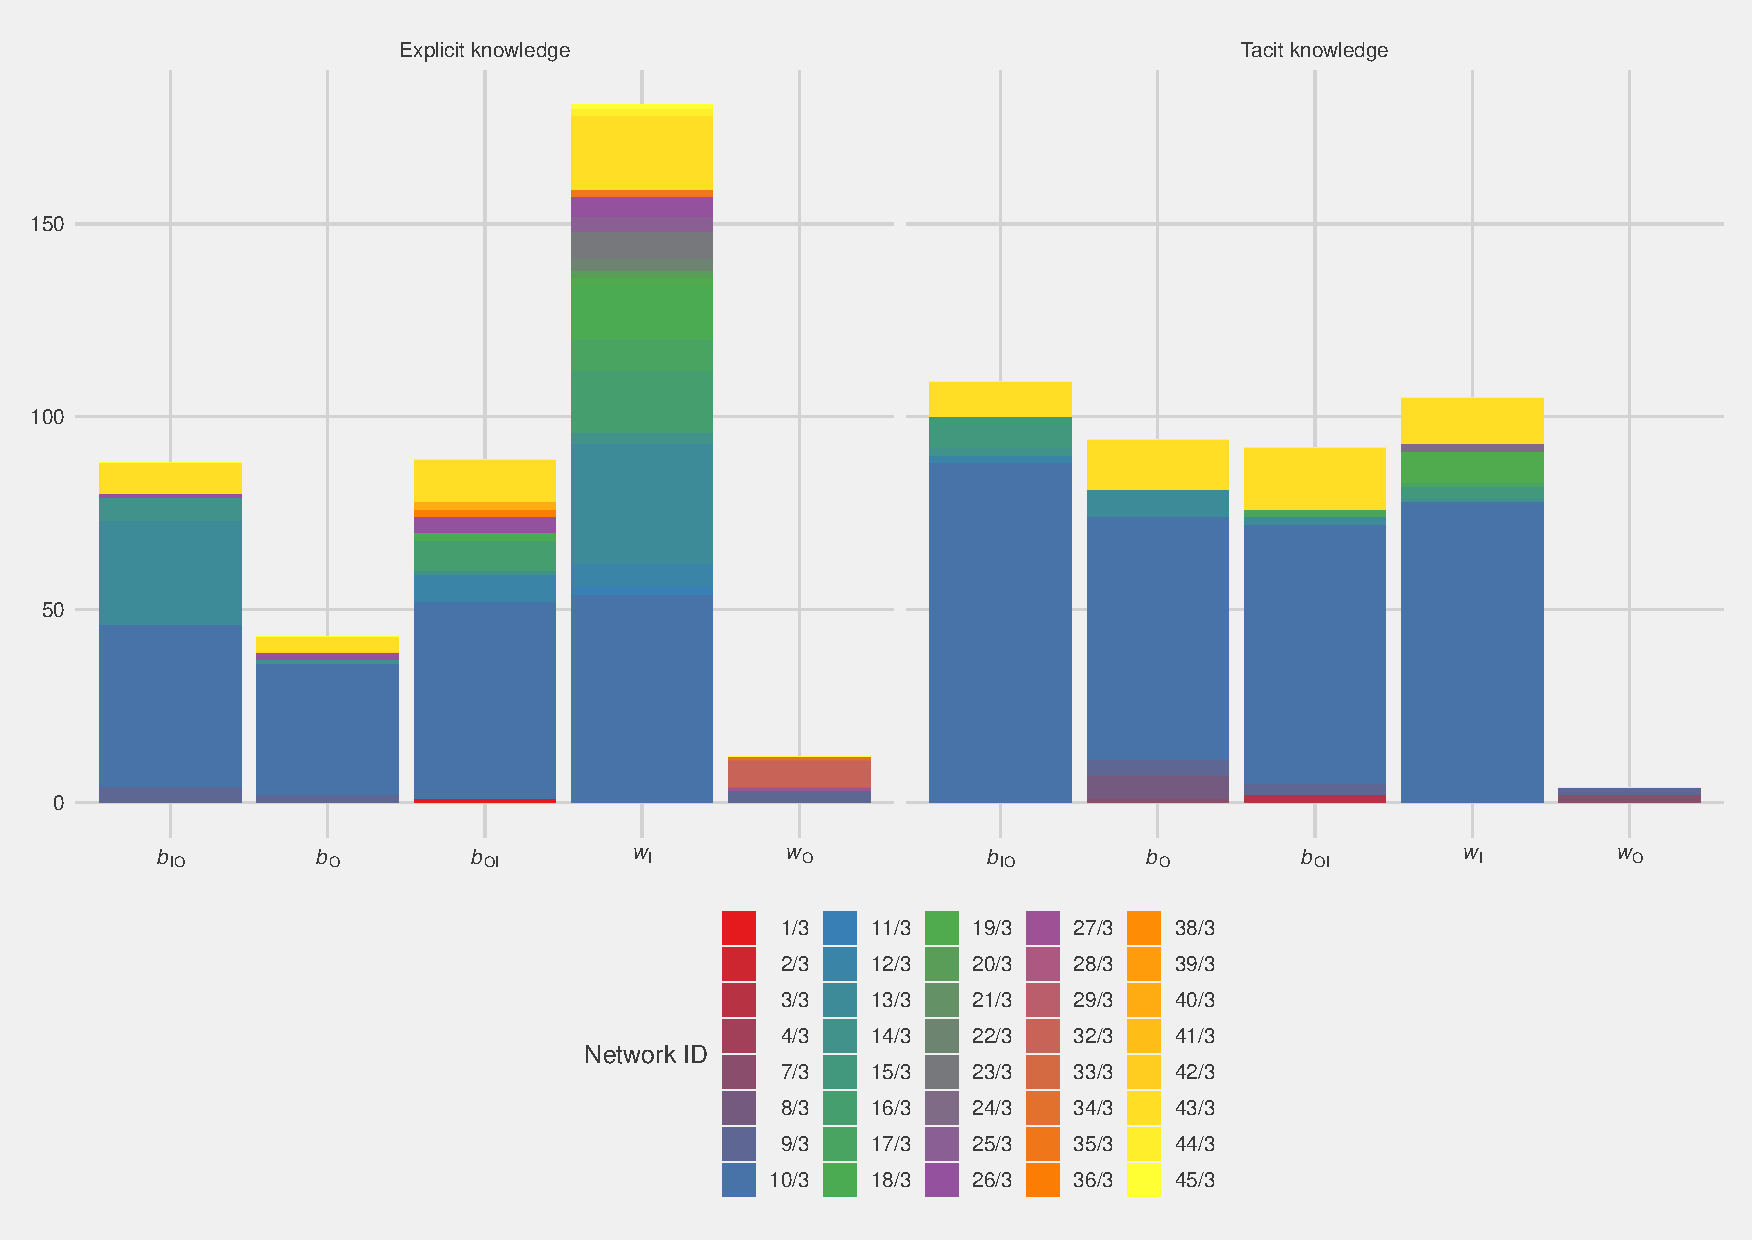
\includegraphics[width = \textwidth]{Images/gf_case3.pdf}
\caption[Raw broker role counts by participant in Case 3]{Raw broker role counts by participant in Case 3. Counts were generated by the \texttt{sna} package in \texttt{R} \citep{butts2016sna}. Note $w_I$ = internal coordinator role, $b_O$ = liaison role, $b_{OI}$ = gatekeeper role, $b_{IO}$ = representative role, and $w_O$ = itinerant broker role. As with the other two cases, the itinerant broker role hardly features. Participant 10/3 stands out as a dominant broker, especially in the tacit knowledge network.}
\label{fig:gf_c3}
\end{figure}

\subsection{Analysis of interview transcripts}

Table \ref{tab:case_3_codes} lists the most frequently referenced codes in each category for Case 3. As with Cases 1 and 2, participants appear to be motivated by an innate need to become more competent and perform meaningful work. Narrow perspectives and superior attitudes often characterised tensions between technical advancement and the scientific agenda. The mechanism that seems to affect knowledge sharing the most is poor communication. As expected with any global initiative, dealing with foreign cultures and the tyranny of distance are other mechanisms affecting knowledge sharing. Organisational boundaries and resource constraints also impact knowledge sharing. Actions that stand out are managing expectations, people acting in their self-interest, efforts to codify tacit knowledge, goal-setting and tapping external expertise. Unmet expectations did feature strongly in the interviews.

\begin{sidewaystable}[hbtp]
\centering
\caption{Most frequently referenced codes in each category: Case 3.}
\label{tab:case_3_codes}
\resizebox{\textwidth}{!}{%
\begin{tabular}{lllc}
\toprule
Category code & Provisional code & Detailed code & References \\ 
\midrule
Innate needs & Seeking autonomy & Becoming more competent &   3 \\ 
Innate needs & Doing satisfying work & Performing meaningful work &   2 \\ 
Innate needs & Seeking autonomy & Connecting with others &   1 \\ 
Internalised social norms & Expressing a particular worldview & Maintaining a narrow perspective &  11 \\ 
Internalised social norms & Identifying with a distinct group & Being absolutely committed to the partnership &   2 \\ 
Internalised social norms & Expressing a particular worldview & Demonstrating a superior attitude &   1 \\ 
Mechanisms \& structures & Spanning real and perceived boundaries & Communicating poorly &  19 \\ 
Mechanisms \& structures & Spanning real and perceived boundaries & Dealing with foreign cultures &  12 \\ 
Mechanisms \& structures & Spanning real and perceived boundaries & Lacking resources &   7 \\ 
Mechanisms \& structures & Spanning real and perceived boundaries & Organisational boundaries &   7 \\ 
Mechanisms \& structures & Building trust relations & Having open and honest discussions &   6 \\ 
Action & Fostering collaboration & Managing expectations &  28 \\ 
Action & Fostering collaboration & Acting in self-interest &  27 \\ 
Action & Applying knowledge innovatively & Breaking new ground &  12 \\ 
Action & Promoting a learning culture & Codifying knowledge &  10 \\ 
Action & Fostering collaboration & Working towards a common goal &   9 \\ 
\bottomrule
\end{tabular}
}
\end{sidewaystable}

\subsubsection{Innate needs}

Given the partnership was dominated by people with a research background, autonomous motivation is bound to feature strongly in Case 3. People who pursue a career in research tend to be autonomously motivated \citep{ryan2014work,suominen2021gold}. The desire to perform meaningful work and master new technology was a significant personal motivator in Case 3:

\begin{quote}
\small
\enquote{I love to learn new things and this is the good thing from the project for sure.} \\
\rightline{\rm --- Participant 9/3}
\end{quote}

\begin{quote}
\small
\enquote{After a very long breakaway from computer systems engineering I'm back working with embedded systems. So this is actually beneficial because it's a change in pace away from just pure software engineering and web applications, and it diversifies and expands my skill-set.} \\
\rightline{\rm --- Participant 16/3}
\end{quote}

\begin{quote}
\small
\enquote{With this project I have a more intimate contact with a different kind of technology and the [importance] for me is that I can adapt [the] technology in my ... for my [research interest].} \\
\rightline{\rm --- Participant 39/3}
\end{quote}

A couple of participants interviewed indicated they were motivated by a strong desire to perform meaningful work. Experiencing meaningful work reflects a deep personal connection between a person and their work, which motivates them to go above and beyond the normal requirements of their work \citep{van2018motivational}. One of the participants expressed his desire to perform meaningful work this way:

\begin{quote}
\small
\enquote{This is one of the reasons I joined [the national research agency] was that for me it was a good job doing interesting work on real science projects that are going to deliver a real benefit. And this project is actually one of those projects. If it's successful it will deliver real benefit, not just locally or nationally, but globally. So that actually makes it quite exciting -- the discovery of new things, that's enjoyable and exciting.} \\
\rightline{\rm --- Participant 16/3}
\end{quote}
 
 Another participant enjoyed interacting with people from across the world. Not only did this make her work more meaningful, it also appears to have satisfied an innate need for social connectedness:
 
 \begin{quote}
\small
\enquote{I think a lot of the people that are involved are very enthusiastic, so, particularly the ones overseas. They've come to visit, and I've gone to Brazil, and it's been nice to see the staff working in the field elsewhere. And have the people come from Mexico to visit, and talk with them, and that's probably been the most enjoyable part.} \\
\rightline{\rm --- Participant 13/3}
\end{quote}

We see a consistent theme emerging across all three cases: participants are generally motivated by a desire to feel competent and perform meaningful work and are thus more likely to be open to learning. The ERGM analysis backs this assertion, where receivers of tacit knowledge tend to have higher levels of autonomous motivation.

\subsubsection{Internalised social norms}

Narrow perspectives and attitudes suggesting a sense of superiority often characterised tensions between technical advancement and the scientific agenda:

\begin{quote}
\small
\enquote{I think that the technical advancement in some ways bounds the scientific agenda ... sometimes technical advancement is slower than the science community would like ... there's a perception among scientists that the technical stuff should just be simple because it's not science ... it's just engineering and anyone can do that.} \\
\rightline{\rm --- Participant 16/3}
\end{quote}

The project leader and lead software engineer from the team driving the initiative believe that many scientists are too focused on their area of expertise or risk averse. They think scientists feel tremendous pressure to compete with others in their field and are reluctant to take risks as their ability to attract funding depends on their track record of delivering successful research outcomes:

\begin{quote}
\small
\enquote{Scientists are competing for small discoveries, and trying to publish a paper that shows a small conclusion about a specific topic. And doing that of course, they end up losing the big picture of what they can achieve if they join forces. And I think this is what is missing ... } \\
\rightline{\rm --- Participant 10/3}
\end{quote}

\begin{quote}
\small
\enquote{We largely see in science these days small incremental improvements and that's largely because the corporate and scientific community in the western societies now has become very risk averse. So people are ... their funding is tied to success, so they're reluctant to take big risks to think outside the box to try something completely different, and so they just do little incremental improvements on what's already known.} \\
\rightline{\rm --- Participant 16/3}
\end{quote}

These comments suggest the partnership was struggling to gain traction. Some of the participating scientists either did not appreciate the challenge of building a cloud-based data analytics platform or were hesitant to try something different that could detract from their ability to attract ongoing research funding. It appears that many of the scientists involved in this partnership (and there were many scientists, see Figure \ref{fig:demographics}) view technology in purely functional terms and not as a crucial enabler of new scientific approaches. This narrow perspective has contributed to a schism between technologists and scientists.

\subsubsection{Social mechanisms \& structures}

The main social mechanisms affecting knowledge flows in Case 3 include poor communication, dealing with foreign cultures, organisational boundaries, limited funding, and the tyranny of distance (Table \ref{tab:case_2_codes}). The interviews suggest geography was a major factor affecting communication. Too much reliance on email communication was an issue:

\begin{quote}
\small
\enquote{Communication also, it's one of the, it brings a lot of boundaries as well, because we are so inefficient in the way we write, email is not necessarily the best tool for us to exchange information, so we need to talk, and that changes completely, because visual communication helps so much. You need to be aware that emails can be misunderstood, there are many other aspects. And there are the acquired aspects of the barrier. Somebody's not talking, but the body language is telling you so much, or the science tells you a lot, the person just went quiet, what's going on? So there is something going on there.} \\
\rightline{\rm --- Participant 10/3}
\end{quote}

The partnership was managed using a hub-and-spoke model. All communication went through the national research agency. This approach meant that partners were reliant on centrally coordinated dissemination of information to know what others were doing:

\begin{quote}
\small
\enquote{I guess we're the centre, and then they're all the nodes. And when it gets a little bit bigger, if it gets bigger, then there will be annual, bi-annual meetings where we'll all get together on Skype or something, and introduce everyone to each other, 'cause a lot of the groups don't know each other.} \\
\rightline{\rm --- Participant 13/3}
\end{quote}

\begin{quote}
\small
\enquote{It appears that the group here at [the national research agency] are acting as a central hub.  So it’s basically a hub and spoke model, or a star model – however you want to describe it – we're the hub, and each collaborator is a node at the end of a spoke.  And there is ... between Mexico and Brazil I think there might be some cross-communication, but largely information comes back to us and then gets disseminated out to people who might need it.  So it's ... we've become like the centralised information broker.} \\
\rightline{\rm --- Participant 16/3}
\end{quote}

\begin{quote}
\small
\enquote{I don't know that any of it is deliberate, it's just that everybody's got particular instructions of what they're meant to be doing, and some of them aren't aware of the background, or aren't aware of who else was operating in the space. And so, yeah, there was just some unusual things that have been happening.} \\
\rightline{\rm --- Participant 22/3}
\end{quote}

For a hub-and-spoke model to work well requires the hub to be very effective at disseminating information. Some participants did not always perceive the national research agency as an effective communicator. Failing to follow up on email communication was an issue:

\begin{quote}
\small
\enquote{Between the two of our groups, when we have an issue we send an email, maybe it gets a reply, maybe it doesn't. And when [the national research agency] needs something they send an email, maybe it gets a reply, maybe it doesn't. There's  no ongoing conversation really happening.} \\
\rightline{\rm --- Participant 41/3}
\end{quote}

Language was also a significant barrier to effective communication. Not all the participants felt comfortable conversing in English, and they were less open as a consequence:

\begin{quote}
\small
\enquote{For sure, for sure it is because all Portuguese-speaking people are involved and not everyone here has good English and they are afraid, they want to but they don't know how to expose and even to understand the other opinions and contributions from English-speaking people.} \\
\rightline{\rm --- Participant 9/3}
\end{quote}

Support for the global partnership was patchy within the national research agency. Although the initiative generated a considerable amount of positive media attention for the agency, the team driving the initiative ran out of money to progress things. The agency did not provide ongoing financial support, despite senior people being aware that the technology needed further development:

\begin{quote}
\small
\enquote{Early on we believed that the technology that was being developed would eventually get us to the point where we could actually track bees as they moved around, or gather that information so that we could access that sort of information. But at the time, the sensors were giving us information on when bees left and returned to a hive, which was a starting point but was never meant to be the end point.} \\
\rightline{\rm --- Participant 22/3}
\end{quote}

\begin{quote}
\small
\enquote{Well we haven't got a budget anymore.  We haven't got any money, so it makes it very difficult to progress relationships with kits, give ... apart from the fact they're not developed yet. But even if they were we haven't got any money, so we have no operational money left.} \\
\rightline{\rm --- Participant 13/3}
\end{quote}

Efforts to secure additional funding appear to have been disjointed. The national research agency has several business units, each representing a different research capability. Each business unit has its own dedicated business development team. This initiative involved data scientists, sensor technologists, software engineers, entomologists, and environmental scientists from several business units. It seems the different business development teams struggled to work together:

\begin{quote}
\small
\enquote{The different sets of business directors or business support people all looking to do things around the global initiative. And so there are things that we discover after the event that are happening, that certainly aren't being shared. So there is certainly no cohesive [business development] happening around the global initiative from my point of view.} \\
\rightline{\rm --- Participant 22/3}
\end{quote}

Those responsible for business development within the agency did not seem particularly motivated to secure additional funding:

\begin{quote}
\small
\enquote{I don't understand why [an agency business unit] were even involved, and their business development person, and two years, talked a lot but did nothing. And now they've gone and we were meant to be assigned another one, and I haven't seen any progress out of that.} \\
\rightline{\rm --- Participant 13/3}
\end{quote}
 
Perhaps the lack of motivation has something to do with how people responsible for business development are rewarded. They receive significant performance bonuses when landing high-value external contacts. Securing funding may not have been deemed not worthwhile. The lack of funding meant that the team behind the initiative was unable to ramp things up. Instead of strengthening relatively new relationships, the project leader needed to seek additional funding. He even considered crowd-funding but this approach was over-ruled by senior managers at the national research agency. One senior manager thought the technology was oversold:

 \begin{quote}
\small
\enquote{I think there’s a bit of overselling of what the current technology package can do in the context of honey bee health.} \\
\rightline{\rm --- Participant 22/3}
\end{quote}
 
 Unmet expectations appeared to give rise to resentment that ultimately hampered knowledge sharing between partners. The project coordinator commented:

\begin{quote}
\small
\enquote{I think there could be a lot more progress, but I think relationships and finance, and all of that is hampering any progress. I think if there was more progress there would be more knowledge sharing, but everyone's still just trying to get off the ground.} \\
\rightline{\rm --- Participant 13/3}
\end{quote}

She was frustrated by people with strong egos in the national research agency getting in the way of progress. They appeared to be more interested in self-promotion than working together in a collaborative manner: 

\begin{quote}
\small
\enquote{Because it's all based on personality and ego, not on the end goal. If I was in the business of hiring and firing I'd just sack them all. As it's really... it's just ridiculous.} \\
\rightline{\rm --- Participant 13/3}
\end{quote}

Operating at a global scale did impact knowledge exchange mechanisms and the emergence of informal social structure. The hub-and-spoke model used to coordinate activities was divisive and hindered wider communication. Relying on email communication does not seem to be an effective way to build trust or engage in open and honest discussions. The geographic spread of participants and lack of funding limited opportunities for face-to-face social interaction, essential for building trust, reaching consensus and exchanging tacit knowledge. 

\subsubsection{Actions}

Failure to manage expectations, people acting out of self-interest, efforts to codify knowledge, trying to get people to work towards a common goal, and tapping external expertise are key actions that influenced the way the global partnership operated. The partnership was launched with great fanfare and attracted global media attention. Unfortunately, the technology for tracking bee movements in and out of hives was still being developed. Partners signed on to the initiative expecting the technology to work out of the box. Teething problems caused some participants to become disillusioned:

\begin{quote}
\small
\enquote{I'm a little worried because I went for this one year ago and we didn't have so far an example of the final thing working. We just say [to our principals] the equipment [is capable] but we need something ready, working, at the final stage, as soon as possible.} \\
\rightline{\rm --- Participant 9/3}
\end{quote}

\begin{quote}
\small
\enquote{I think the promise always was that the sensors and the technology was all well developed and straightforward and all you needed was to pick up the sensors and apply them to your bees and do a bit of programming and everything would work.} \\
\rightline{\rm --- Participant 22/3}
\end{quote}

It seems many of the participants did not fully appreciate the technical challenge of building a cloud-based data management system with limited resources:

\begin{quote}
\small
\enquote{I think that there's a perception amongst the scientists that the technical stuff should just be simple because it's not science, right? It's just engineering and anyone can do that and crank the handle, and they don't really understand the challenges involved in building the technical solution that they're looking for.} \\
\rightline{\rm --- Participant 16/3}
\end{quote}

Expectations may have been more realistic had there been more effective communication. The hub-and-spoke model did not allow partners to easily share their experience of getting the technology to work. Disappointment in the technology gave rise to concern about possible reputational damage to the national research agency. This concern may explain why internal support for the global partnership did not eventuate in some instances:

\begin{quote}
\small
\enquote{I was getting concerned about our international profile and whether we were going to be ... I was just worried about all these groups overseas who might know honeybees but don't know technology too much and whether they're going to be pissed off by the [agency] product.} \\
\rightline{\rm --- Participant 22/3}
\end{quote}

Even though some partners were disappointed the technology did not meet expectations, they did not have to pay for technology starter kits and were motivated to join the partnership to further their own research interests:

\begin{quote}
\small
\enquote{It came from scientists around the world and from beekeepers, asking to have access to the technology that we have developed at [the national research agency]. They became aware of that because of a media campaign we have done, and a result of that huge exposure from the media, they became aware of the research, and they started looking at how can they work with us, because they have a number of questions they would like to answer using this technology.} \\
\rightline{\rm --- Participant 10/3}
\end{quote}

\begin{quote}
\small
\enquote{I guess we benefit in the sense that we get access to technology that would have been very difficult to access earlier and I guess that's true of anybody who’s partnering with [the national research agency]. It's very hard to get, even just to buy the RFID chips, it's quite difficult, if you're buying less than one million of them. So it works from a logistics sense to have everybody working together on that front. And then [the agency] obviously benefits in the sense that it gets the data from everybody who's working in the [partnership].} \\
\rightline{\rm --- Participant 41/3}
\end{quote}
 
One of the goals of the partnership was to develop a standardised data repository. Everybody would provide or access data in a standard format. Because scientists wanted to collect data to answer specific research questions, agreeing to a standardised way of collecting and managing data proved quite challenging. Each partner wanted a custom setup that suited their way of thinking, which was at odds with the idea of performing big data analytics on a common data set. Unlike the other two cases, there was no proper commitment to a common objective:

\begin{quote}
\small
\enquote{The original idea was that everyone would do the same experiments using the same protocols with the same equipment so that everything would be standardised and we could do comparative analysis. It became apparent very quickly that that wasn't going to be the way things worked, because each partner has strong opinions on what science they would like to do.} \\
\rightline{\rm --- Participant 16/3}
\end{quote}

Partners also seemed reluctant to share their data with others, fearing that others would publish their results before them. It appears they were wary of each other and not particularly open or trusting:

\begin{quote}
\small
\enquote{And so there's some reluctance to share data because someone might just take your data and publish it before you. And I guess that's a trust issue, and that takes time for them to decide that that's not going to happen in this case.} \\
\rightline{\rm --- Participant 16/3}
\end{quote}

To facilitate the sharing of know-how, the team driving the global partnership set up a project wiki to allow participants to capture their learnings. The idea was that partners would update the wiki, but it seems not everyone bought into this idea. One of the team members driving the initiative wrote up most of the experimental setups used by partners. Partners kept their know-how confined to their group or preferred to describe experimental setups in their publications:

\begin{quote}
\small
\enquote{I'm a person who likes to formalise and document stuff, and the reason behind that is if I can formalise and document stuff, then that becomes a resource for those people and I can make that available to them and they can have a look at it any time that they want ... so I've done all the experimental set up documentation, this experiment was run from this date to this date, it used these pieces of equipment, they were configured in this way, they were placed in these locations, those sorts of things.} \\
\rightline{\rm --- Participant 16/3}
\end{quote}

\begin{quote}
\small
\enquote{If you really have something that could help other people in the future we try to describe the protocols in publications.} \\
\rightline{\rm --- Participant 9/3}
\end{quote}

\begin{quote}
\small
\enquote{Generally [knowledge sharing is] practised within our group that any work that we do, we keep details and instructions so somebody else could do it. And so that helps quite a lot with sharing the ... sharing knowledge within our group.} \\
\rightline{\rm --- Participant 41/3}
\end{quote}

The person who championed the wiki realised it was not the most effective tool for knowledge sharing. He felt it did not facilitate open discussion or idea generation and was keen to try something different:

\begin{quote}
\small
\enquote{I'm of the opinion that the current wiki approach is not conducive to knowledge sharing ... it's not conducive to knowledge sharing, it’s too static and it's ... you've got discrete little bundles of knowledge that are spread across multiple pages within the wiki: it doesn't facilitate discussion. I guess we could set it up to run a forum which is one of my suggestions, I think there should be an open forum between the collaborators where they feel ... where they don't feel intimidated to ask any questions.} \\
\rightline{\rm --- Participant 41/3}
\end{quote}

The senior manager was critical of the leadership of the global partnership. He thought the team driving the initiative had not succeeded in setting out a common vision that everybody could aspire to:

\begin{quote}
\small
\enquote{If we're going to have something that we want to call a \enquote{global initiative}, we'd have to ensure that everybody is on-board with a common vision from the start, and I think we have to seriously look at the leadership skills of those that we expect to lead. So I think we could do better there.} \\
\rightline{\rm --- Participant 22/3}
\end{quote}

Despite the tension stemming from unmet expectations, poor communication, vested interests, and issues around leadership, much learning took place. Partners were exposed to new technology and needed to figure out how to tag various bee species more efficiently. The team building the data repository gained insight into what bee researchers were most interested in, which helped improve the overall system design:

\begin{quote}
\small
\enquote{It could be the entomologists, or the other scientists, can be the people developing the hardware, it's the same approach with either, it's like well we've discussed this, we know that we need to do this. In order to do that I need the following information because I need this kind of detail, and I'll provide answers, and then from there I'll go OK, given that, well then there’s a whole range of implicit assumptions [...] which are these, these, these, and these. Are they correct?  These are the correct assumptions or is there something I've missed here?} \\
\rightline{\rm --- Participant 16/3}
\end{quote}

Although the evidence suggests many of the scientists were frustrated with the technology not working as expected, some were still excited by the prospect of being able to collaborate with other scientists on a global scale: 

\begin{quote}
\small
\enquote{So working together, if people respect the collaboration of different expertise at the end of the reports I think it's not a problem.  I think it's the way when we have a huge project like that with different goals from different places and working together, at the end we're going to have a beautiful job that only could be done by a big group of researchers and expertise in different parts of the world, and maybe different species of bees too.} \\
\rightline{\rm --- Participant 9/3}
\end{quote}

Judging by the reported actions of participants, it seems commitment to work towards a common goal was lacking. Many participants appear to have acted in their self-interest. Not getting participants to agree on a common goal was considered a failure of leadership. Using a wiki to capture learning was also not particularly effective. There was some acknowledgement that face-to-face interaction is better for sharing experiences. Despite these issues, some participants remained committed to the idea of scaling data collection efforts worldwide to understand bee behaviour better.

\subsection{Case synopsis}

Case 3 was struggling to get off the ground. Despite being launched with great fanfare and attracting interest from bee researchers worldwide, the national research agency was unwilling to invest much in the global partnership for honeybee research. The team driving this initiative was not given sufficient resources to progress things. Unmet expectations resulted in growing resentment among some partners. The hub-and-spoke management model also meant the team driving the initiative operated as significant gatekeepers. Partners were unable to interact directly with each other, limiting the exchange of tacit knowledge. Disseminating information via email and the wiki proved to be an ineffective form of communication. Language barriers did not help communication either. One can attribute some of the dysfunction in the global partnership to partners who put their personal research interests ahead of the broader project goals. While many partners were happy to take advantage of free access to technology, they were quick to complain when it did not work \enquote{out of the box}. \medskip

Nonetheless, participants did learn how to use the new technology and probably developed a greater appreciation of the technical difficulty of setting up a centralised data repository. The team behind the global partnership appears to have under-estimated the challenge of managing a global partnership. This case exemplifies how structure shapes perceptions, behaviour, and action in open innovation projects. 

\section{Chapter conclusion}

The critical realist approach used in this study employed quantitative social network analysis to observe social reality in three open innovation partnerships (referred to as the \enquote{empirical} level of reality). In this chapter, qualitative analysis provided insights into the unobserved social reality in each partnership (the \enquote{actual} level of reality). Provisional codes, derived from the theoretical propositions developed in Chapters 2 and 3, were expanded into detailed codes by applying inductive logic to semi-structured interview transcripts. The logic of retroduction was applied to the detailed codes to group these into category codes aligned with the main components of \citeauthor{loyal2001agency}'s \citeyearpar{loyal2001agency}  agency model. The qualitative analysis aimed to examine how agency and structure were affected by innate needs, internalised norms, social mechanisms and structures, and actions in each partnership. \medskip

The qualitative analysis reveals that levels of openness vary considerably in Case 1. Participants do not enjoy equal access to critical information and know-how. There is significant gatekeeping, which appears to be driven by perceptions of trustworthiness and judgements about the absorptive capacity of others. The varying levels of openness and gatekeeping may have negatively impacted agency and thus the emergence of informal structures that support the sharing and application of know-how. We see evidence for this in the sparse number of ties in the tacit knowledge provide network. We can attribute much of this to the gatekeeping by the general manager. The ERGM analysis of broker roles shows that the partners were generally quite willing to share their tacit knowledge (significant and positive effect for the representative broker role effect). Knowledge brokerage did not feature strongly in Case 2. Trust levels among participants were high. The trust stems from partners all being highly committed to achieving a shared goal. There is a clear understanding of the importance of maintaining healthy relationships to that end. Participants were comfortable sharing ideas and knowledge and reflecting on what works or does not work. There seem to have been very few constraints on agency. The relatively dense tacit knowledge provider network indicates a well-developed informal structure supporting the sharing and application of know-how in Case 2. Interviewees were less optimistic in Case 3, pointing to significant internal tensions. Several factors hampered tacit knowledge exchanges in this case. Unlike in Case 2, the geographic spread of participants in Case 3 was a significant issue and negatively impacted the emergence of informal structures that support the sharing and application of know-how. We see strong evidence of gatekeeping in the ERGM analysis of broker roles. This gatekeeping may be the result of the hub-and-spoke model used to coordinate the global partnership. Relying on email and a wiki to disseminate information or knowledge was problematic. Another major issue was the lack of commitment to achieving a shared goal, an indicator of inadequate leadership. \medskip  

The next chapter aims to transform the initial set of seven propositions into more general statements about potential mechanisms for tacit knowledge sharing in open innovation. These more general statements represent the real (knowledge of what and why things are) from a critical realist perspective.

% \begin{landscape}
% \scriptsize
% \singlespacing

% \begin{longtable}[c]{lllccc}

% \caption[Breakdown of codes by case]{Breakdown of code references by case. The breakdown of codes allows one to compare and contrast cases.\label{tab:filtered_codes}} \\
% \toprule
% Category code & Provisional code & Detailed code & Case 1 & Case 2 & Case 3 \\
% \endfirsthead

% \multicolumn{6}{c}{Table \ref{tab:filtered_codes} continued from previous page.}\\
% \toprule
% Category code & Provisional code & Detailed code & Case 1 & Case 2 & Case 3 \\
% \midrule
% \endhead

% \bottomrule \\
% \endfoot

% \bottomrule
% \endlastfoot

% \midrule
% Innate needs & Doing satisfying work & Performing meaningful work &   6 &   3 &   2 \\ 
% Innate needs & Seeking autonomy & Becoming more competent &   1 &   5 &   3 \\ 
% Innate needs & Seeking autonomy & Connecting with others &   0 &   1 &   1 \\ 
% Internalised social norms & Expressing a particular worldview & Demonstrating a superior attitude &   4 &   1 &   1 \\ 
% Internalised social norms & Expressing a particular worldview & Maintaining a narrow perspective &   6 &   0 &  11 \\ 
% Internalised social norms & Expressing a particular worldview & Navigating change &   3 &   0 &   0 \\ 
% Internalised social norms & Expressing a particular worldview & Over-analysing things &   0 &   2 &   0 \\ 
% Internalised social norms & Identifying with the collaboration & Being absolutely committed &   2 &  19 &   2 \\ 
% Mechanisms \& structures & Building trust relations & Breaking trust &   0 &   4 &   5 \\ 
% Mechanisms \& structures & Building trust relations & Demonstrating credibility &   3 &   8 &   2 \\ 
% Mechanisms \& structures & Building trust relations & Demonstrating swift trust &   9 &   3 &   1 \\ 
% Mechanisms \& structures & Building trust relations & Having open and honest discussions &  11 &  13 &   6 \\ 
% Mechanisms \& structures & Building trust relations & Investing in relationships &  13 &  21 &   3 \\ 
% Mechanisms \& structures & Building trust relations & Showing commitment &   2 &   5 &   0 \\ 
% Mechanisms \& structures & Building trust relations & Taking responsibility &   1 &   2 &   1 \\ 
% Mechanisms \& structures & Building trust relations & Withholding information &   2 &   1 &   1 \\ 
% Mechanisms \& structures & Defining the rules of engagement & Avoiding conflicts &   0 &   0 &   2 \\ 
% Mechanisms \& structures & Defining the rules of engagement & Lacking structure &   0 &   0 &   1 \\ 
% Mechanisms \& structures & Defining the rules of engagement & Playing by the rules &   0 &   0 &   1 \\ 
% Mechanisms \& structures & Encountering power structures & Dealing with large organisations &   8 &   9 &   0 \\ 
% Mechanisms \& structures & Encountering power structures & Exercising control &   0 &   0 &   1 \\ 
% Mechanisms \& structures & Protecting knowledge & Engaging in subversive behaviour &   0 &   3 &   0 \\ 
% Mechanisms \& structures & Protecting knowledge & Protecting intellectual property &   7 &   9 &   3 \\ 
% Mechanisms \& structures & Protecting knowledge & Withholding information &   3 &   1 &   2 \\ 
% Mechanisms \& structures & Spanning real and perceived boundaries & Communicating poorly &   8 &   3 &  19 \\ 
% Mechanisms \& structures & Spanning real and perceived boundaries & Dealing with change &   4 &  14 &   0 \\ 
% Mechanisms \& structures & Spanning real and perceived boundaries & Dealing with foreign cultures &   0 &  12 &  12 \\ 
% Mechanisms \& structures & Spanning real and perceived boundaries & Dealing with the tyranny of distance &   3 &  13 &   6 \\ 
% Mechanisms \& structures & Spanning real and perceived boundaries & Gaining access to key people &   9 &   0 &   3 \\ 
% Mechanisms \& structures & Spanning real and perceived boundaries & Lacking resources &   3 &   1 &   7 \\ 
% Mechanisms \& structures & Spanning real and perceived boundaries & Organisational boundaries &   4 &   3 &   7 \\ 
% Mechanisms \& structures & Spanning real and perceived boundaries & Overcoming disciplinary boundaries &   0 &   3 &   4 \\ 
% Mechanisms \& structures & Spanning real and perceived boundaries & Recognising and managing boundaries &   0 &   1 &   1 \\ 
% Mechanisms \& structures & Spanning real and perceived boundaries & Working with different personalities &   0 &   2 &   4 \\
% Action & Applying knowledge in practice & Dealing with complexity &  10 &   3 &   7 \\ 
% Action & Applying knowledge in practice & Improving practices &  30 &   6 &   0 \\ 
% Action & Applying knowledge in practice & Interacting face-to-face &   9 &   0 &   5 \\ 
% Action & Applying knowledge in practice & Practising integrated thinking &   0 &   4 &   3 \\ 
% Action & Applying knowledge in practice & Reflecting on what can work &   3 &  15 &   8 \\ 
% Action & Applying knowledge in practice & Relying on tacit knowledge &   0 &   1 &   5 \\ 
% Action & Applying knowledge in practice & Using data to guide decisions &   9 &   0 &   0 \\ 
% Action & Applying knowledge in practice & Working in different contexts &   2 &   3 &   7 \\ 
% Action & Applying knowledge innovatively & Breaking new ground &   1 &  19 &  12 \\ 
% Action & Applying knowledge innovatively & Demonstrating a can-do attitude &   0 &   2 &   0 \\ 
% Action & Applying knowledge innovatively & Profiting from innovation &   5 &  20 &   0 \\ 
% Action & Applying knowledge innovatively & Rising to the challenge &   0 &   8 &   0 \\ 
% Action & Connecting people & Acting as a company representative &   0 &  14 &   1 \\ 
% Action & Connecting people & Coordinating people &   0 &   0 &   1 \\ 
% Action & Connecting people & Excluding others &   0 &   0 &   6 \\ 
% Action & Connecting people & Forging strong stakeholder relations &   0 &   1 &   0 \\ 
% Action & Connecting people & Gatekeeping &  11 &   1 &   4 \\ 
% Action & Connecting people & Practising liaison brokerage &  17 &   1 &   2 \\ 
% Action & Connecting people & Resolving conflicts &   0 &   1 &   0 \\ 
% Action & Empowering others & Empowering customers &   4 &   0 &   0 \\ 
% Action & Empowering others & Negotiating from a position of strength &   3 &   0 &   0 \\ 
% Action & Empowering others & Sharing knowledge with others &   1 &   8 &   1 \\ 
% Action & Fostering collaboration & Acting in self-interest &   4 &   2 &  27 \\ 
% Action & Fostering collaboration & Embracing multidisciplinarity &   3 &   3 &   4 \\ 
% Action & Fostering collaboration & Ensuring everyone benefits &   2 &   2 &   5 \\ 
% Action & Fostering collaboration & Having difficult conversations &   2 &   3 &   1 \\ 
% Action & Fostering collaboration & Having sufficient critical mass &   0 &   1 &   1 \\ 
% Action & Fostering collaboration & Managing expectations &   2 &   5 &  28 \\ 
% Action & Fostering collaboration & Operating in different geographic markets &   1 &   0 &   0 \\ 
% Action & Fostering collaboration & Supporting others &   3 &   1 &   4 \\ 
% Action & Fostering collaboration & Understanding customers &   3 &   0 &   1 \\ 
% Action & Fostering collaboration & Working in isolation &   0 &   0 &   6 \\ 
% Action & Fostering collaboration & Working towards a common goal &   8 &  15 &   9 \\ 
% Action & Promoting a learning culture & Codifying knowledge &   0 &   2 &  10 \\ 
% Action & Promoting a learning culture & Fostering a learning culture &   2 &   0 &   0 \\ 
% Action & Promoting a learning culture & Gaining a broader understanding &  16 &   4 &   6 \\ 
% Action & Promoting a learning culture & Learning by doing &   0 &  26 &   8 \\ 
% Action & Promoting a learning culture & Taking short cuts &   0 &   0 &   1 \\ 
% Action & Promoting a learning culture & Tapping external expertise &  15 &  13 &   8 \\ 

% \end{longtable}

% \end{landscape}